%Author: Miguel Duarte (http://miguelduarte.pt), updated by Fernando Brito e Abreu
%IEEE ISCTE-IUL Student Branch (http://ieee-iscteiul.org)

\documentclass[a4paper, 12pt, oneside]{thesis} %twoside
\usepackage{graphicx}
\usepackage{verbatim}
\usepackage[utf8]{inputenc}
\usepackage[T1]{fontenc}
\usepackage[portuguese, english]{babel}
\usepackage{pdfpages}
\usepackage{time}
\usepackage{appendix}
\usepackage{sidecap}
\usepackage[super]{nth}
 
\usepackage{lipsum}  
\usepackage{makecell}
\usepackage{threeparttable}
\usepackage{url}
\usepackage{amsmath, amssymb, amsthm}

\usepackage{tabularx,booktabs,ragged2e}
\newcolumntype{L}{>{\RaggedRight\arraybackslash}X}
  

\usepackage{url}
\usepackage[]{algorithm2e}
\usepackage{rotating}
\usepackage{multirow}
\usepackage{listings}
\usepackage{amsmath}
\usepackage{amsfonts}
\usepackage{amssymb}
\usepackage{pgfplots}
\usepackage{graphicx}
\usepgfplotslibrary{statistics}
\usetikzlibrary{patterns}
\usepackage{comment}
\usepackage{pgfplotstable}
\usepackage{float}


%--------------------------------------------------
% Adicionado para ter cor nas tabelas
\usepackage{colortbl}
%
%--------------------------------------------------
%
% Adiciona o estilo do capítulo
\usepackage{titlesec, color}
\definecolor{gray75}{gray}{0.75}
\newcommand{\hsp}{\hspace{20pt}}
%\titleformat{\chapter}[hang]{\Huge\bfseries\scshape}{\thechapter\hsp\textcolor{gray75}{|}\hsp}{0pt}{\Huge\bfseries}
%
%--------------------------------------------------
% Formatação das páginas 
\pagestyle{fancy}
\fancyhf{}
\fancyhead[LE,RO]{\slshape \leftmark}

%\fancyfoot[LE,RO]{\thepage}


\fancypagestyle{plain}{% % <-- this is new
  \fancyhf{} 
  \fancyfoot[LE,RO]{\thepage} % same placement as with page style "fancy"
  \renewcommand{\headrulewidth}{0pt}}
  \renewcommand{\chaptermark}[1]{\markboth{\thechapter.\ #1}{}}
%
%--------------------------------------------------
%  
% Package para ter glossário
\usepackage[nonumberlist]{glossaries} % glossário sem numeração das páginas em que aparecem as siglas
\makeglossaries
%\robustify{\gls}
%
%--------------------------------------------------
% Package para ter índice de equações
\usepackage{tocloft}
\makeatother
% Criar a listas de equações
\numberwithin{equation}{chapter}
\setcounter{secnumdepth}{3}
%
%--------------------------------------------------

\newcommand*\rfrac[2]{{}^{#1}\!/_{#2}}
\newcommand{\tuple}[1]{\langle #1\rangle}
\newcommand{\fromRoot}[1]{./data/#1}

\def \listfigures {List of Figures}

\def \university {University Institute of Lisbon}

\def \department {Department of Information Science and Technology}

\def \supervisortitle {Supervisor}
\def \supervisorname {Your Supervisor's Name, Assistant or Associate or Full Professor}
\def \supervisoruniv{ISCTE-IUL}

%Se tiverem co-orientador basta descomentar esta parte seguinte

%\def \cosupervisortitle {Co-supervisor}
%\def \cosupervisorname {Your Co-supervisor's Name, Assistant or Associate or Full Professor}}
%\def \cosupervisoruniv {FCT/UNL}

\def \dissertationstatement {Dissertation in partial fulfillment of the requirements for the degree of}
\def \dissertationtitle {M.Sc. in Computer Science and Business Management}

\begin{document}
\newtheorem{mydef1}{Definition}
\selectlanguage{english}

\frontmatter

\title {
    Using Syntax Highlighting to Improve OCL to Model Comprehension\\
    }
\authors{Maria Pedro dos Santos Sales}
            
%\addresses  {\groupname\\\deptname\\\univname}

\def \supervisortitle {Supervisor}
\def \supervisorname {Fernando Brito e Abreu, PhD, Associate Professor}
\def \supervisoruniv{DCTI/Iscte}

\def \cosupervisortitle {Co-supervisor}
\def \cosupervisorname {Marina Alexandra Pedro Andrade, Assistant Professor}
\def \cosupervisoruniv {DM/Iscte}

\date       {November, 2020}
\subject    {Subject}
\keywords   {keyword 1;keyword 2; keyword 3}
\maketitle



\fancyfoot[LE,RO]{\thepage}

\pagestyle{fancy}
%%------Página de Citação (opcional)-----
%caso não queiram citação, removam esta parte
\pagestyle{empty}

\null\vfill
\textit{"Some people never go crazy. What truly horrible lives they must lead."}

\begin{flushright}
Charles Bukowski
\end{flushright}

\vfill\vfill\vfill\vfill\vfill\vfill\null
\cleardoublepage 

%-------RESUMO---------
%mesmo se escreverem a tese em inglês, tem que haver um resumo/abstract em português
%MPSS%\addtotoc{Resumo}

Modelos, metamodelos e transformações de modelo desempenham um papel central no Desenvolvimento Dirigido por Modelos (MDD). A Linguagem para Especificação de Restrições em Objetos (OCL) foi inicialmente proposta como parte da Linguagem de Modelagem Unificada (UML) para adicionar os recursos de precisão e validação que faltavam nestes diagramas, e também para expressar regras de boa formação no metamodelo. A OCL possui outras aplicações, tais como definir métricas de desenho, modelos de geração de código ou regras de validação para transformações de modelo, exigidas em MDD. 

Aprender OCL como parte de um curso de UML na universidade parecia portanto natural. No entanto não é o que se verifica. Acreditamos que isso se deva principalmente a uma percepção generalizada de que OCL é difícil de aprender, tendo em conta afirmações feitas na literatura. Com base em dados recolhidos em anos letivos anteriores de um grande número de alunos de licenciatura de diferentes cursos de Engenharia de Software, analisámos como a aprendizagem por cláusulas contratuais de UML + OCL se compara a vários outros tópicos do SWEBOK. O resultado do processo de aprendizagem foi recolhido de forma rigorosa, apoiada por uma plataforma de e-learning. Realizámos estatísticas inferenciais sobre os dados para apoiar as nossas conclusões, de forma a identificar as variáveis explicativas relevantes para o sucesso / fracasso dos alunos. As conclusões obtidas levaram-nos a estender uma ferramenta OCL existente com dois recursos novos: o primeiro é voltado para os estudantes de OCL e vai direto ao núcleo da questão, permitindo visualizar como as expressões OCL percorrem um diagrama de classes UML; o segundo é voltado para investigadores e permite calcular métricas de complexidade OCL, habilitando a réplica de um estudo como este.

% Palavras-chave do resumo em Português
\begin{keywords}
OCL; UML; Realce do modelo; Compreensão do OCL.
\end{keywords}
% to add an extra black line


%-------ABSTRACT---------
%MPSSModels, metamodels and model transformations play a central role in~\gls{mdd}.~\gls{ocl} was initially proposed as part of the~\gls{uml} standard to add the precision and validation capabilities lacking in its diagrams, and also to express well-formedness rules in its metamodel. OCL has found several other applications, such as for defining design metrics, code-generation templates or validation rules for model transformations, required in MDD.

Learning OCL as part of a UML course at the university would, therefore, seem natural, but is still the exception rather than the rule. We believe that is mainly due to a widespread perception that OCL is hard to learn, gleaned from claims made in the literature. Based on data gathered over the past school years from a large number of undergraduate students of different Software Engineering courses, we analyzed how learning design by contract clauses with UML+OCL compares with several other~\gls{swebok} topics. The outcome of the learning process was collected in a rigorous setup, supported by an e-learning platform. We performed inferential statistics on that data to support our conclusions, and to identify the relevant explanatory variables for students success/failure. The obtained findings lead us to extend an existing OCL tool with two novel features: one is aimed at OCL apprentices and goes straight to the heart of the matter, by allowing to visualize how OCL expressions traverse a UML~\gls{classDiagram}; the other is intended for researchers and allows to compute OCL complexity metrics, making it possible to replicate a research study like this one.

% Palavras-chave do resumo em Inglês
\begin{keywords}
OCL; UML; Model Highlight; OCL Comprehension.
\end{keywords} 




\setstretch{1.3}

%-------AGRADECIMENTOS---------
%MPSSS%\btypeout{Acknowledgements}
%\addtotoc{Acknowledgements}
%\thispagestyle{plain}
%\chapter*{Acknowledgements}
%\begin{center}{\huge{\textit{Acknowledgements}} \par}\end{center}

\acknowledgements

I want to express my sincere gratitude to my thesis supervisors Prof. Doutor Fernando Brito e Abreu and Prof. Doutora Marina Alexandra Pedro Andrade, for their continuous support, guidance and encouragement. I would also like to thank all the involved professors and students that took part in the experiments and made use of the provided prototypes, which allowed the conclusion of this research.

%\vfil\vfil\null

\cleardoublepage

\pagestyle{fancy}
%-------IDIOMA DA TESE---------
%Descarreguem a versão que disponibilizamos deste template em PT
%se quiserem fazer a tese em PT: http://ieee-iscteiul.org
\selectlanguage{english}
%\selectlanguage{portuguese}

%-------ÍNDICE---------
%\lhead{\emph{Contents}}
\tableofcontents
\cleardoublepage
%-------LISTA DE FIGURAS---------
%\lhead{\emph{List of Figures}} 
\listoffigures 
\cleardoublepage
%-------LISTA DE Tabelas---------
%\lhead{\emph{List of Tables}} 
\listoftables 
\cleardoublepage
%-------LISTA DE ALGORITMOS (caso necessário)---------
%\lhead{\emph{List of Algorithms}}
%\addtotoc{List of Algorithms}
%\listofalgorithms
%\listoftables

\setstretch{1.5}
\clearpage

%-------Glossário---------

%\newglossaryentry{metamodel} {
    name={Metamodel},
    description={
    A simplified version of a model
    }
}
\newglossaryentry{classDiagram} {
    name={Class Diagram},
    description={
    A class diagram in the UML is a static structure diagram that describes the structure of a system, showing it's classes, attributes, operations, and the relationships among objects
    }
}
\newglossaryentry{objectDiagram} {
    name={Object Diagram},
    description={
    An object diagram in the UML is a structural diagram that shows an instance of a system in a particular point in time
    }
}
\newglossaryentry{stateDiagram} {
    name={State Diagram},
    description={
    A state diagram in the UML is a behavioral diagram that describes the different states of a system
    }
}
\newglossaryentry{formalMethods} {
    name={Formal Methods},
    description={
    Kind of mathematical technique to specify, develop and verify software and hardware systems
    }
}
\newglossaryentry{componentDiagram} {
    name={Component Diagram},
    description={
    Describes the several components of a system, how they are organized and wired
    }
}
\newglossaryentry{fleschKincaidGradeLevel} {
    name={Flesch-Kincaid Grade Level},
    description={
    Readability tests developed by the US Navy that conferes a U.S. grade level score.
    }
}
\newglossaryentry{gunningFogIndex} {
    name={Gunning Fog Index},
    description={
    Readability formula that estimates the degree of education needed to understand a given text, from a scale from 0 to 20. A value of 8 classifies the text as readable for someone in the Eighth grade, and above 17 for a graduate level
    }
}
\newglossaryentry{colemanLiauIndex} {
    name={Coleman-Liau Index},
    description={
    Readability formula that indicates the necessary U.S grade level to comprehend a text
    }
}
\newglossaryentry{smogIndex} {
    name={SMOG Index},
    description={
    ‘Simple Measure of Gobbledygook’ (SMOG) Index measures the number of years of education a person needs to have to understand a text
    }
}
\newglossaryentry{automatedReadabilityIndex} {
    name={Automated Readability Index},
    description={
    Readability formula that indicates the necessary U.S grade level to comprehend a text. The difference of this metric lays on the fact that it counts characters, rather than syllables, and also counts sentences
    }
}
\newglossaryentry{facade} {
    name={Facade},
    description={
    Structural software-design pattern that hides the underlying system complexities by providing an interface to the client
    }
}


%
% Adiciona o estilo do capítulo
\titleformat{\chapter}[hang]{\Huge\bfseries\scshape}{\thechapter\hsp\textcolor{gray75}{|}\hsp}{0pt}{\Huge\bfseries}

%-------CAPÍTULOS---------
\mainmatter	  % Numeração normal (1,2,3...)

%chapter 1
\newcommand{\novathesis}{\emph{novathesis}}
\newcommand{\novathesisclass}{\texttt{novathesis.cls}}

%%%%%%%%%%%%%%%%%%%%%%%%%%%%%%%%%%%%%%%%%%%%%%%%%%%%%%%%%%%%%%%%%%%%%%%%%%%%%
%% This is the code to include document PARTs
%% and in the back of the PART page includes an graphic about the document 
%% structure
%\partcover{Fundamentals}{part1.pdf}
%{This Part covers the motivation, scope, research problems and main contributions of this work and highlights the fundamental topics, such as: Software Development Process, Software Analytics and Process Mining. It also presents a Systematic Literature Review about Software Development Analytics in Practice.}
%%%%%%%%%%%%%%%%%%%%%%%%%%%%%%%%%%%%%%%%%%%%%%%%%%%%%%%%%%%%%%%%%%%%%%%%%%%%%%

\chaptercover{Introduction}{chap:Introduction}
{This chapter describes the motivation and scope of this dissertation and presents the contributions and the organization of the document.}
%%%%%%%%%%%%%%%%%%%%%%%%%%%%%%%%%%%%%%%%%%%%%%%%%%%%%%%%%%%%%%%%%%%%%%%%%%%%%%

%\chapterquotes{...All things -from the tiniest virus to the greatest galaxy- are, in reality, not things at all, but processes...}{In \textit{"Future Shock"}, 1970.}{Alvin Toffler(1928-2016)}{American writer, futurist, and businessman known for his works discussing modern technologies, including the digital and the communication revolutions, with emphasis on their effects on cultures worldwide.}

UML~\cite{uml2005} was created by the~\gls{omg}~\cite{omg2017} and had its first specification draft proposed in January 1997. It's currently the standard language used in software development for specifying, visualizing, assembling, and documenting artefacts of software systems. However, UML graphical modelling constructs are not precise enough to express all relevant aspects of a specification. In order to mitigate this problem, a semi-formal language named OCL~\cite{ocl2014} was included in the UML standard and has been employed in a beneficial way to provide precision to models~\cite{Gogolla2004}. OCL is based on first-order logic (\emph{predicate calculus}) and set theory, provides many collection operations and can be used in several contexts, such as expressing constraints (class invariants, pre-and post-conditions, ...) and derivation rules for attributes or associations in a Class Diagram, specifying well-formedness rules and metrics at the~\gls{metamodel} level, querying objects in an~\gls{objectDiagram} (equivalent to~\gls{sql} queries in relational databases), and specifying guards on state transitions in a~\gls{stateDiagram}.

\gls{formalMethods} is a long-discussed topic in Software Engineering, and several studies have been conducted to assess the benefits of using OCL alongside UML models~\cite{Briand2004}~\cite{Briand2005}. Albeit there are still disputes about under what circumstances formal methods and languages should be used, there appears to be a consensus that OCL is advantageous to modellers once they overcome the initial learning curve, which has been proven as a difficult task~\cite{Zamansky2016}.

\section{Motivation and research problem}
\label{sec:Introduction-Motivation}

Several support tools were developed to assist in MDD, including the analysis and design phases where modellers need to interpret and write OCL expressions. These tools have their specific characteristics and provide a variety of useful functionalities, including syntactic analysis, connection with the UML model, and debugging~\cite{Toval2003}. To the best of our knowledge, none of these tools provides syntax highlighting in a Class Diagram for manually introduced OCL expressions, which we believe that could soften the learning curve for this language by reducing the mental burden when reading, analyzing and writing expressions. Our hypothesis is based on the multiple studies available that investigate the impact of visual aspects (colour, layout, font, ...) on program comprehension, and they all reveal positive outcomes on subject's comprehensibility when enhancing programs with visual features~\cite{Rambally1986}~\cite{Yusuf2007}~\cite{Mehta2009}~\cite{Sarkar2015}.

\section{Objectives}
\label{sec:Introduction-Objectives}

As a first objective, we aim to shed some light on which factors influence OCL's learning process. To achieve this, we study the results of OCL-related questionnaires taken by bachelor students across different school years, and how distinctive variables affect their results, including the complexity of the questions (given by readability indices), and the complexity of the answers (given by OCL complexity metrics). 

As the second objective, we seek a solution to soften OCL's learning curve by reducing the cognitive effort needed to correctly produce a clause from a specification in~\gls{nl}, in the context of a UML Class Diagram. To accomplish this goal, we propose the OCL Highlight Plugin (presented in the next section).

\section{Contributions}

\label{sec:Introduction-Contributions}

The contributions of this dissertation are the design, implementation, prototype and experimental validation of two plugins for the~\gls{use} tool. The first plugin, named OCL Highlight Plugin, provides syntax highlighting for manually introduced OCL expressions in the context of a UML class diagram. This plugin analyzes the syntax tree of an OCL expression and highlights the diagram components that are referred in that specific expression, including classes, properties, and navigations. The second plugin, named OCL Complexity Plugin, analyzes the same syntax tree and evaluates the complexity of OCL expressions using a set of metrics defined by Reynoso et al.~\cite{Reynoso2005, Reynoso2010}. The idea of including the calculation of these metrics in a plugin resulted from the studies performed to fulfil the first objective of this dissertation.

\section{Dissertation organization}
\label{sec:Introduction-Organization}

This dissertation is structured in 5 chapters, where the first is the introduction. The remainder of this document is organized as follows. Chapter~\ref{chap:RelatedWork} presents the topic's background and related work, consisting of relevant research contributions. Chapter~\ref{chap:Implementation} describes the implemented prototypes, from a broader perspective to a more detailed one. Chapter~\ref{chap:Results} discusses the conducted experiments and relevant results. Chapter~\ref{chap:Conclusion} contains the concluding remarks and addresses open issues and future research work directions.

%Chapter~\ref{chap:Implementation} describes our implementation of the plugin, from a broader perspective into a more detailed one. Chapter~\ref{chap:Results} discusses the conducted experiment with our solution and relevant results. Chapter~\ref{chap:Conclusion} contains the concluding remarks, also addressing some open
%issues and future research work directions.

%chapter 2
\chaptercover{Related Work}{chap:RelatedWork}
{In this chapter, we explore the concepts and state of the art concerning the topics that relate to our intended work, which allow us to have a better understanding of the problem under study. This chapter is organized in 5 sections, structured as follows. Section~\ref{sec:RelatedWork-ModelDrivenDevelopment} starts by presenting the main concepts of Model-Driven Development, including the definition of UML, and OCL. Section~\ref{sec:RelatedWork-UML} covers existing studies on comprehension of UML Class Diagrams, and the impact of OCL on UML-based development. Section~\ref{sec:RelatedWork-Metrics} discusses the complexity of OCL expressions and presents existing metrics proposed by experts to calculate this complexity. Section~\ref{sec:RelatedWork-SyntaxHighlight} examines relevant papers on the impact of syntax highlighting on program comprehension. Finally, Section~\ref{sec:RelatedWork-OCLTools} presents some OCL support tools and their functionalities.}
%%%%%%%%%%%%%%%%%%%%%%%%%%%%%%%%%%%%%%%%%%%%%%%%%%%%%%%%%%%%%%%%%%%%%%%%%%%%%%

%\chapterquotes{...All things -from the tiniest virus to the greatest galaxy- are, in reality, not things at all, but processes...}{In \textit{"Future Shock"}, 1970.}{Alvin Toffler(1928-2016)}{American writer, futurist, and businessman known for his works discussing modern technologies, including the digital and the communication revolutions, with emphasis on their effects on cultures worldwide.}

To identify all relevant studies for our topic, we started by defining the search strategy, which states that the title, abstract, and keywords of the articles, books, and conference proceedings will be searched in the appropriate electronic databases (IEEE Xplore, ACM Digital Library, Elsevier, Springer, ...) according to the following search~\textit{string}: 

((("uml" AND "class diagram") OR "ocl" OR "program") AND ("comprehension" OR "complexity" OR "highlight")) OR ("ocl" AND "tool")
%((("uml" AND "class diagram") OR "ocl" OR "program") AND ("comprehension" OR "complexity" OR ("eye" AND "tracking") OR "highlight")) OR ("ocl" AND "tool")

To only select articles that are pertinent to our topic, the following inclusion/exclusion criteria were applied: if the abstract of the article is not clearly related with the topic under study, or if it wasn't published by a top publisher (e.g. IEEE, ACM, Wiley, Springer, Elsevier), then the article wasn't considered. Additionally, we used forward snowballing whenever the references of the selected articles were relevant in the context of this dissertation.

\section{Concepts of Model-Driven Development} 
\label{sec:RelatedWork-ModelDrivenDevelopment}

Model-Driven Development is presented as the methodology of software development with models as the primary focus, rather than computer programs. Models are artefacts used to specify the system's required functionality and architecture and to guide the development of the final piece of software. Since these models are closer to the problem domain, abstracted from the underlying technologies, they are a high-level specification, easier to specify, understand and maintain~\cite{mda2014}~\cite{Selic2003}~\cite{Atkinson2003}.

To express the necessary information of a system, models need to be represented in a way that can be comprehended by modellers, developers, stakeholders, and other supporting systems. A modelling language is either a graphical or textual computer language that allows the creation of models, following a specific set of structures, terms, notations, syntaxes, semantics, and integrity rules~\cite{mda2014}. There are many well-known modelling languages, including~\gls{bpmn}, SQL Schema,~\gls{xml} Schema, and UML~\cite{uml2005}. UML is currently accepted as the standard graphical notation for software development, but its diagrams cannot express all constraints and essential aspects of a system precisely. To address the existing flaws in UML diagrams, IBM proposed Object Constraint Language~\cite{ocl2014}, which is now part of the UML standard. OCL is a "semi-formal" language since it lacks inference mechanisms (second-order logic), that allows specification of invariants, pre-and post-conditions as well as the description of guards and constraints on operations.

\section{UML Class Diagrams comprehension} 
\label{sec:RelatedWork-UML}

Over the years, several studies have been conducted to assess how software engineers build, understand, and design programs. In the topic of program comprehension, we're particularly interested in addressing how humans process class diagrams to acquire information about a system. Class Diagrams, which are one type of UML diagrams, describe the structure and global behaviour of a program by showing it's classes, attributes, operations, and relationships, hence this type of diagram is useful for both modelling and understanding of a program.  
Guehénéuc~\cite{Gueheneuc2006} and Yusuf~\cite{Yusuf2007} used eye-tracking technology to obtain data on how subjects process UML Class Diagrams, namely how they explore, visualize and examine data. Sight is the most important sense in this process, which makes it relevant to study the behaviour of the human eye. Three types of information are particularly relevant: fixations, saccades, and scanpaths. Fixations are defined by a period of time where the subject maintains the visual gaze on a single location, represented by a pair of coordinates; saccades involve a quick movement between two fixation points; finally, scanpaths are defined as directed paths formed by saccades between fixations. Results of eye-tracking studies can be represented as shown: Figure \ref{fig:01_gazeplot} shows a gaze plot of a UML class diagrams with fixations, saccades, and scanpaths, whereas Figure~\ref{fig:02_heatmap} shows a heatmap of fixations. By analyzing these two figures, it's possible to discern the path taken by the subject's eyes through the diagram and which were the main focus points. This information is important when trying to understand how subjects visually process class diagrams. Relevant conclusions show that relationships mainly contain fixations on its ends and saccades on the line, indicating that lines are mainly used for navigation purposes. A large number of fixations on a \textit{stimulus}, an object that is viewed by a subject, indicate a greater effort to understand the object in question, due to either its complexity or the poor layout arrangement. The use of colour information was found useful for experts when trying to explore class diagrams more efficiently.

%\plot{chapter6/chapter6-1.pdf}[ProcessLabs Portfolio covers Software Development Process Mining][9][H][trim=0cm 0cm 0cm 0cm]

\begin{figure}[ht]
\centering
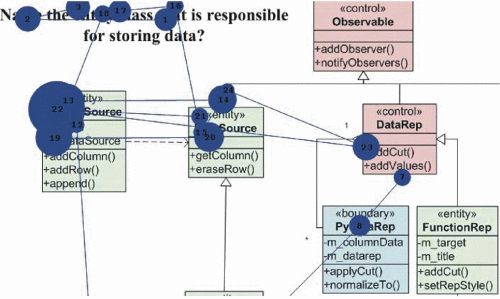
\includegraphics[width=0.7\textwidth]{Template/Chapters/figures/4_RelatedWork/01_GazePlot.png}
\caption{Gaze plot of a UML class diagram exploration~\cite{Yusuf2007}}
\label{fig:01_gazeplot}
\end{figure}

\begin{figure}[ht]
\centering
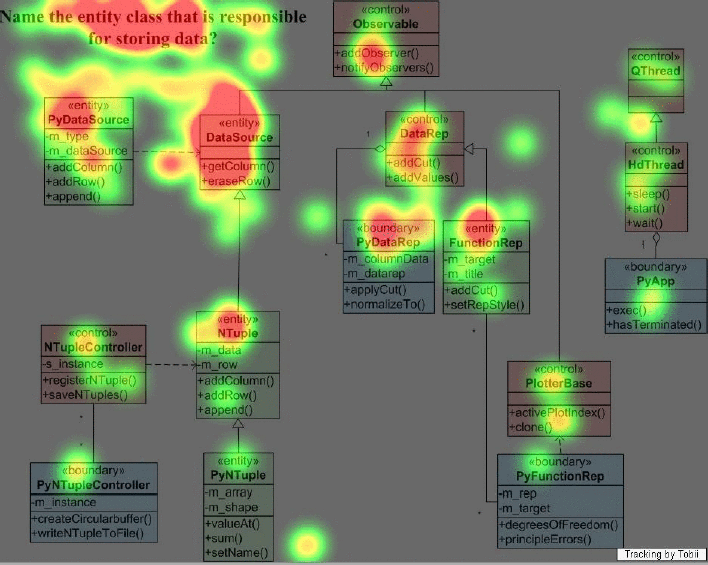
\includegraphics[width=0.7\textwidth]{Template/Chapters/figures/4_RelatedWork/02_HeatMap.png}
\caption{Heatmap of a UML class diagram exploration~\cite{Yusuf2007}}
\label{fig:02_heatmap}
\end{figure}

Comprehension of UML Class Diagrams is particularly important when designing and maintaining OCL expressions because they're always tied to the context of this type of diagram. These expressions can be used to specify objects' invariants and pre-and post-conditions on operations, and also to query the system data to return information to the user. The impact of OCL in UML-based development has been discussed throughout many investigations over the past years, focusing on OCL's influence on comprehension and maintainability of UML models, and whereas the additional effort and formality justify the benefit. Briand et al. ~\cite{Briand2004,Briand2005} investigated the impact of OCL during development, understanding, and modification of UML analysis documents, which are three typical software engineering activities. The authors compared subjects (\nth{4} year software/computer engineering students) performance on comprehension and maintenance tasks when using OCL to document invariants, pre-and post-conditions, which are typically documented in NL. Results showed that OCL has the potential to promote comprehension and modification of UML diagrams, but requires a high level of experience and training.

\section{Metrics for OCL expressions} 
\label{sec:RelatedWork-Metrics}

The cognitive effort needed to comprehend, design, and/or maintain systems is influenced by the levels of complexity that characterize OCL expressions. There has been an ongoing effort to define OCL complexity metrics~\cite{Reynoso2005Book}, and to study how they can capture different levels of comprehensibility and maintainability of OCL expressions. Reynoso et al. ~\cite{Reynoso2005, Reynoso2010} pursued insight in the process of understanding OCL expressions by applying the techniques of chunking (which involves recognizing groups of declarations and the extraction of information, that is remembered as a chunk) and tracing (which involves scanning through a program in different directions in search of relevant chunks). While there are many distinct metrics that capture different aspects that affect expression's complexity, these authors decided to focus on the impact of tracing-based metrics, because this technique was proven as an essential activity in program comprehension~\cite{Reynoso2005Book}. They found statistical significance on the impact of tracing-related metrics on the understandability and, consequently, modifiability of OCL expressions. The process is shown in Figure~\ref{fig:03_oclcomplexity}: the structural properties of an OCL expression affect the cognitive complexity needed to comprehend that expression, which consequently influences understandability and maintainability. Table~\ref{tbl:tracingMetrics} shows the metrics in question and their classifications, depending on their focus on the structural properties of OCL expressions: coupling (degree of interdependence between objects), size, and length.

\begin{figure}[ht]
\centering

\includegraphics[width=0.9\textwidth]{Chapters/figures/4_RelatedWork/03_OCLComplexity.png}
\caption{Relationship between structural properties of an OCL expression, cognitive complexity related to tracing, understandability and maintainability (based on~\cite{Reynoso2005Book})}
\label{fig:03_oclcomplexity}
\end{figure}

%\begin{table}[ht]
\centering
\begin{threeparttable}  
\caption{Tracing-related OCL expression metrics (based on~\cite{Reynoso2005Book})}
\label{tbl:tracingMetrics}
\begin{tabular}{@{}lll@{}}
\toprule
\begin{tabular}[c]{@{}l@{}}Metric \\ Acronym\end{tabular} & \begin{tabular}[c]{@{}l@{}}Metric \\ Description\end{tabular}                                                      & \begin{tabular}[c]{@{}l@{}}Metric \\ Classification\end{tabular} \\ \midrule
NNR                                                       & Number of Navigated Relationships                                                                                  & C                                                                \\
NAN                                                       & Number of Attributes referred through Navigations                                                                  & C                                                                \\
WNO                                                      & \begin{tabular}[c]{@{}l@{}}Weighted Number of referred Operations \\ through Navigations\end{tabular}              & C                                                                \\
NNC                                                       & Number of Navigated Classes                                                                                        & C                                                                \\
WNM                                                       & Weighted Number of Messages                                                                                        & C, S                                                             \\
NPT                                                       & \begin{tabular}[c]{@{}l@{}}Number of Parameters whose Types are classes\\  defined in a class diagram\end{tabular} & C                                                                \\
NUCA                                                      & Number of Utility Classes Attributes Used                                                                          & C                                                                \\
NUCO                                                      & Number of Utility Classes Operations Used                                                                          & C                                                                \\
DN                                                        & Depth of Navigations                                                                                               & L                                                                \\
WNN                                                       & Weighted Number of Navigations                                                                                     & S                                                                \\
WCO                                                       & Weighted Number of Collection Operations                                                                           & S                                                                \\ \bottomrule
\end{tabular}
\begin{tablenotes}
    \small
    \item Note: In the table above, C stands for Coupling, S stands for Size, and L stands for Length.
\end{tablenotes}
\end{threeparttable} 
\end{table}

\begin{table}[ht]
\centering
\begin{threeparttable}  
\caption{Tracing-related OCL expression metrics (based on~\cite{Reynoso2005Book})}
\label{tbl:tracingMetrics}
\begin{tabular}{@{}lll@{}}
\toprule
\begin{tabular}[c]{@{}l@{}}Metric \\ Acronym\end{tabular} & \begin{tabular}[c]{@{}l@{}}Metric \\ Description\end{tabular}                                                      & \begin{tabular}[c]{@{}l@{}}Metric \\ Classification\end{tabular} \\ \midrule
NNR                                                       & Number of Navigated Relationships                                                                                  & C                                                                \\
NAN                                                       & Number of Attributes referred through Navigations                                                                  & C                                                                \\
WNO                                                      & \begin{tabular}[c]{@{}l@{}}Weighted Number of referred Operations \\ through Navigations\end{tabular}              & C                                                                \\
NNC                                                       & Number of Navigated Classes                                                                                        & C                                                                \\
WNM                                                       & Weighted Number of Messages                                                                                        & C, S                                                             \\
NPT                                                       & \begin{tabular}[c]{@{}l@{}}Number of Parameters whose Types are classes\\  defined in a class diagram\end{tabular} & C                                                                \\
NUCA                                                      & Number of Utility Classes Attributes Used                                                                          & C                                                                \\
NUCO                                                      & Number of Utility Classes Operations Used                                                                          & C                                                                \\
DN                                                        & Depth of Navigations                                                                                               & L                                                                \\
WNN                                                       & Weighted Number of Navigations                                                                                     & S                                                                \\
WCO                                                       & Weighted Number of Collection Operations                                                                           & S                                                                \\ \bottomrule
\end{tabular}
\begin{tablenotes}
    \small
    \item Note: In the table above, C stands for Coupling, S stands for Size, and L stands for Length.
\end{tablenotes}
\end{threeparttable} 
\end{table}


The definition of these metrics is described below, based on~\cite{Reynoso2005Book}:

\begin{definition}\label{def:NNR}
NNR Metric (Number of Navigated Relationships): Measures the total number of navigated relationships in an expression. Relationships are only counted once, even if they're navigated multiple times.
\end{definition}

\begin{definition}\label{def:NAN}
NAN Metric (Number of Attributes referred through Navigations): Counts the number of attributes referred through navigations.
\end{definition}

\begin{definition}\label{def:WNO}
WNO Metric (Weighted Number of referred Operations through navigations): Measures the sum of weighted operations (where the weight is defined by the number of \textit{in/out} parameters,  including the return type) mentioned through navigations.
\end{definition}

\begin{definition}\label{def:NNC}
NNC Metric (Number of Navigated Classes): Measures the number of classes, association classes or interfaces referred through navigations.
\end{definition}

\begin{definition}\label{def:WNM}
WNM Metric (Weighted Number of Messages): This metric is defined as the sum of weighted messages (where the weight is defined by the number of parameters) present in an expression.
\end{definition}

\begin{definition}\label{def:NPT}
NPT Metric (Number of Parameters whose Types are classes defined in the class diagram): This metric is particularly used in pre- and post-conditions, and it counts the number of different classes and interfaces used as \textit{in/out} parameters or result.
\end{definition}

\begin{definition}\label{def:NUCA}
NUCA Metric (Number of Utility Class Attributes used): Measures the number of utility classes' attributes used in an expression. Attributes that belong to the same utility class are only counted once, even if they're referred multiple times.
\end{definition}

\begin{definition}\label{def:NUCO}
NUCO Metric (Number of Utility Class Operations used): This metric definition is similar to the NUCA metric, but instead of attributes it considers operations.
\end{definition}

\begin{definition}\label{def:DN}
DN Metric (Depth of Navigations): Measures the maximum depth of a navigation tree, where the root node represents the class name of the contextual instance (\textit{self}). For each navigation that starts from \textit{self}, we create a branch that connects to a new node, which represents the navigated class. A new tree is created if a navigation contains a collection operation defined in terms of new navigation(s), and it's connected to the original tree through a “definition connection”.
\end{definition}

\begin{definition}\label{def:WNN}
WNN Metric (Weighted Number of Navigations):  This metrics is defined as the sum of weighted navigations presented in an expression, where the weight is defined by the level on which the operation is used in an expression.
\end{definition}

\begin{definition}\label{def:WCO}
WCO Metric (Weighted Number of Collection Operations): Measures the sum of weighted collection operations, where the weight is defined by the level on which the operation is used in an expression.
\end{definition}

Later in this document (subsection~\ref{Results-OCLComplexityMetrics}), we present the results of our investigation on the influence of these metrics on the success/failure of bachelor students when answering OCL questionnaires. We decided to include as a contribution of this dissertation a plugin for Bremen's USE tool~\cite{use} that allows modellers to evaluate OCL expressions and get the calculated complexities given by these metrics. The implementation details are described in section~\ref{chap:Implementation-OCLComplexityPlugin}.

\section{Impact of syntax highlighting on program comprehension}
\label{sec:RelatedWork-SyntaxHighlight}

In the context of this dissertation, it is not only important to understand what affects the comprehensibility of UML Class Diagrams and OCL expressions, but also to investigate the effort that has been made to improve program comprehension. The tasks of understanding and maintaining software systems are greatly influenced by the levels of readability and comprehensibility of programs. These can be affected by many factors, including naming scheme, indentation, commenting, and documentation. This section focuses on relevant research findings on the impact of syntax highlighting in program readability and comprehension. Syntax highlighting is a feature present in several text editors that allow displaying text in different colours (including background colour) and fonts depending on its categorization, making it easily distinguishable from other types of text without affecting the behaviour of the code. Figure~\ref{fig:06_syntaxhighligh1} shows the same code snippet with and without syntax highlight. On the right side the important keywords, e.g. \textit{while} or \textit{print}, and the comment are easily detected, comparing to the rest of the code, because they are displayed in different colours.

\begin{figure}[ht]
\centering
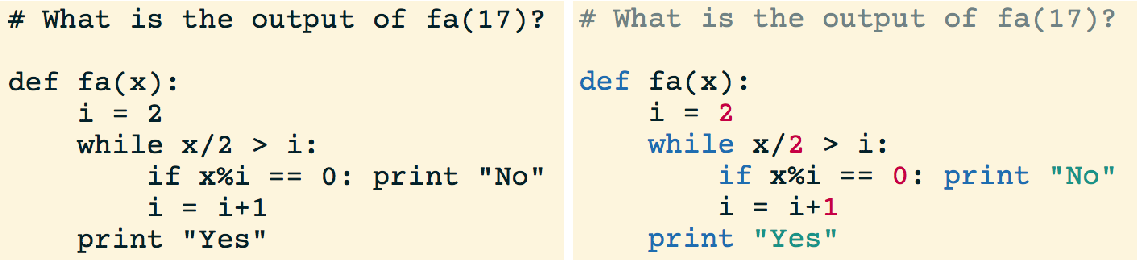
\includegraphics[width=0.9\textwidth]{Chapters/figures/4_RelatedWork/04_SyntaxHighlight1.png}
\caption{Same code with (right) and without (left) syntax highlighting~\cite{Sarkar2015}}
\label{fig:06_syntaxhighligh1}
\end{figure}

Initial studies were mainly concerned with the effect of colours on program comprehension in order to facilitate the learning process and increase developers' productivity, as the majority of tools was only available in black and white. Rambally~\cite{Rambally1986} studied the effect of two colour schemes on program comprehension when compared to a version of the same program presented in black and white: Color-scheme-A used different colours for code blocks, e.g. loops and conditionals; Color-scheme-B used different colours to identify statements and functions, e.g. I/O (Input/Output), decision and declaration statements, and variable binding. From a sample of 44 intermediate-level (novice) and 35 senior-level (expert) programming students, results showed that, in general, both groups could better understand programs when using Color-scheme-B. An interesting note mentioned in this experiment is that the participants subjectively favoured Color-scheme-A as the easiest to understand, even tough results supported Color-scheme-B as the most effective for the completion of the given comprehension tasks.

Several years after this research, Sarkar~\cite{Sarkar2015} did an experiment to evaluate the impact of syntax colouring on program comprehension time, using ten graduate computer science students. Even though the experiment's validity is threatened by the small number of participants, it showed that assignments were solved remarkably faster when using syntax highlighting. The author collected the participants' sessions with an eye-tracking device and discerned that syntax highlighting directed participants' focus on to smaller regions of the code (see Figure~\ref{fig:06_syntaxhighligh2}). In some cases, even some keywords were completely ignored, as seen in Figure~\ref{fig:06_syntaxhighligh3}. Another interesting remark taken from this investigation is that the benefits of syntax highlighting in novice programmers are significantly more relevant when compared to experienced programmers, which might indicate that it's a useful feature when learning a certain language, but less important for using it.

\begin{figure}[ht]
\centering
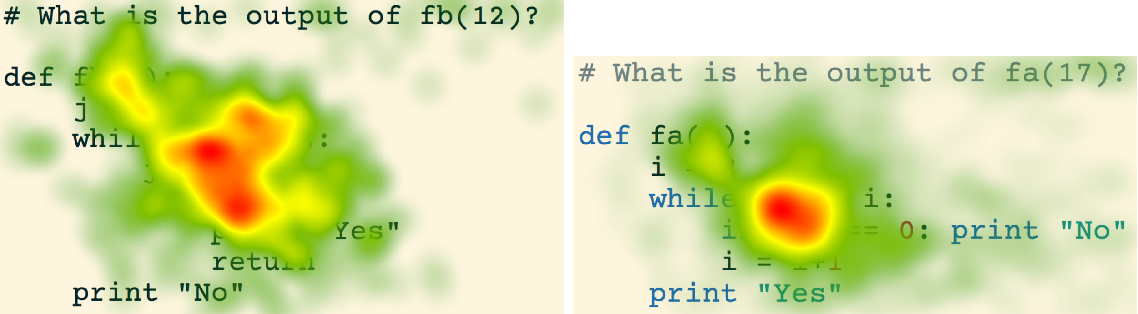
\includegraphics[width=0.9\textwidth]{Chapters/figures/4_RelatedWork/04_SyntaxHighlight2.png}
\caption{Fixation heat map for the same code without (left) and with (right) syntax highlighting~\cite{Sarkar2015}}
\label{fig:06_syntaxhighligh2}
\end{figure}

\begin{figure}[ht]
\centering
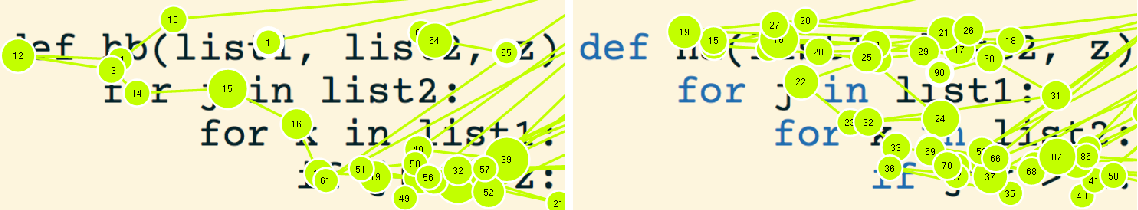
\includegraphics[width=0.9\textwidth]{Chapters/figures/4_RelatedWork/04_SyntaxHighlight3.png}
\caption{Gaze plot for the same code without (left) and with (right) syntax highlighting. The numbers represent the order in which the fixations occurred~\cite{Sarkar2015}}
\label{fig:06_syntaxhighligh3}
\end{figure}

An important aspect when using syntax highlighting is to decide which features to include and how to code them. It's essential to determine which is the most efficient way to display certain information, e.g. choosing to use colour X over Y for a specific category of information, selecting a background colour instead of a text colour, ... Mehta and Zhu~\cite{Mehta2009} focus on the effect of colours (red and blue) on cognitive task performance. They start by describing the theory defended by colour theorists which states that people create specific associations to colours depending on the repeated situations they experience with that colour: red is an intensive colour normally associated with errors or dangers, while blue is mostly associated with calmness, peace, and tranquillity. Results from this research show that distinct colours offer different benefits, and the choice of the right colour depends on the nature of the task. As red primarily activates an avoidance motivation, it mainly enhances performance on detail-oriented tasks. On the other hand, blue activates an approach motivation which is more beneficial for creative tasks.

In summary, previous research shows that visual coding hints through syntax highlighting can improve program comprehension, and consequently reduce the time needed to complete a given task, especially for novice developers. Many distinct features can be used (e.g. colour, font size, ...), but it's important to understand the different effects they provoke on people so that we can choose the appropriate feature depending on the desired outcome. As one of the main goals of this dissertation is to soften OCL's learning curve, we developed a second plugin for USE, this time providing syntax highlight to the elements of a UML Class Diagram referenced by an OCL expression. The implementation details are presented in section~\ref{chap:Implementation-OCLHighlightPlugin}, and the experiments of it's success described in subsection~\ref{chap:Results-OCLHighlightPlugin}.

\section{OCL tools}
\label{sec:RelatedWork-OCLTools}

Currently, there are several OCL tools available, either freely or for commercial use, that assist modellers in the development, analysis, and maintenance of systems. It's important to investigate their main functionalities to understand what this dissertation can offer to the current body of knowledge. Toval et al. ~\cite{Toval2003} defined a set of features found desirable when working with OCL and presented a comparison of the main characteristics (shown in Table~\ref{tbl:oclToolsCharacteristics}) of the existing tools. In the meantime, some of them received updates (for example, to support newer versions of OCL), some had their development cancelled or were integrated into other systems, and other tools emerged. For our topic, we're mainly interested in the available features of the two most common OCL tools, which are USE (UML-based Specification Environment)~\cite{use}, and Eclipse OCL~\cite{eclipseocl}.

\begin{table}[ht]
\centering
\begin{threeparttable}  
\caption{Main OCL tools characteristics (based on~\cite{Toval2003})}
\label{tbl:oclToolsCharacteristics}
\begin{tabular}{@{}lccc@{}}
\toprule
\multicolumn{1}{c}{Analysis}                                 & Communication                                                       & Features                                                                              & \begin{tabular}[c]{@{}c@{}}Dynamic \\ validation\end{tabular}                     \\ \midrule
\begin{tabular}[c]{@{}l@{}}Syntatic \\ analysis\end{tabular} & Model-independent                                                   & \begin{tabular}[c]{@{}c@{}}Guided support \\ for constraint \\ development\end{tabular} & \begin{tabular}[c]{@{}c@{}}Invariant \\ validation\end{tabular}                   \\
\begin{tabular}[c]{@{}l@{}}Type \\ checking\end{tabular}     & \begin{tabular}[c]{@{}c@{}}With connection \\ to model\end{tabular} & \begin{tabular}[c]{@{}c@{}}Code generation \\ from OCL \\ specifications\end{tabular}   & \begin{tabular}[c]{@{}c@{}}Consistent \\ checking \\ of contraints\end{tabular}   \\
                                                             &                                                                     & \begin{tabular}[c]{@{}c@{}}Insertion of \\ OCL expressions*\end{tabular}                 & \begin{tabular}[c]{@{}c@{}}Pre- and \\ post-conditions \\ validation\end{tabular} \\ \bottomrule
\end{tabular}
\begin{tablenotes}
    \small
    \item * Includes three possibilities: imported from a UML model, imported from an independent file or manually introduced.
\end{tablenotes}
\end{threeparttable} 
\end{table}

USE is one of the pioneering OCL tools. It was initially developed in Java by Mark Richters as a dissertation project at the University of Bremen~\cite{Gogolla2007}. It's freely distributed under GPLv2 (GNU General Public License version 2.0), and the latest version, USE 6.0.0, was released in September 2020. Main functionalities include syntactic analysis, type checking, dynamic validation of invariants and pre-and post-conditions, and consistency checking. The core feature of USE is to validate specifications that consist of UML class diagrams and OCL expressions (invariants and pre-and post-conditions), which can be effective when helping modellers and developers in early development stages. It's also important to refer that USE allows the connection with UML models, which is made through a specific file (\textit{.use}). Additional functionalities include an evaluation browser (see Figure~\ref{fig:05_usetool2}), and syntax highlighting of the coverage of the expressions (see Figure~\ref{fig:05_usetool3}). The evaluation browser allows users to manually introduce OCL expressions and to debug them, as it generates an~\gls{ast} from the input text that is evaluated against the model and returns either a syntax error or the result of the given expression. These two features are the most important, in the context of this dissertation, because they provide the basis for the development of the plugin for syntax highlighting when evaluating OCL expressions in the evaluation browser. As a last remark, this tool allows third parties to contribute with additional functionalities through plugins.

\begin{figure}[ht]
  \centering
  \begin{tabular}{@{}c@{}}
    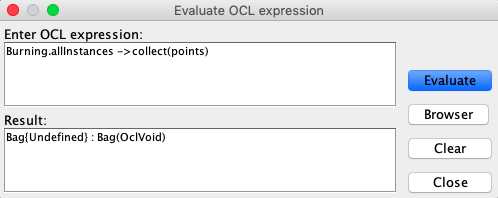
\includegraphics[width=.6\linewidth]{Chapters/figures/4_RelatedWork/05_USETool_1.png} \\[\abovecaptionskip]
    \small (a) Expression evaluation
  \end{tabular}

  \vspace{\floatsep}

  \begin{tabular}{@{}c@{}}
    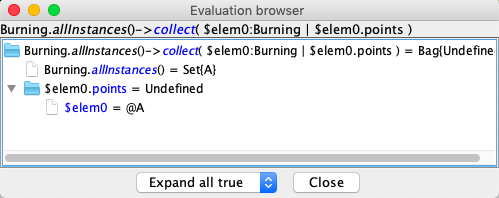
\includegraphics[width=.6\linewidth]{Chapters/figures/4_RelatedWork/05_USETool_2.png} \\[\abovecaptionskip]
    \small (b) Evaluation browser
  \end{tabular}

  \caption{Evaluation browser on USE (Royal and Loyal example from~\cite{Warmer2003})}\label{fig:05_usetool2}
\end{figure}

\begin{figure}[ht]
\centering
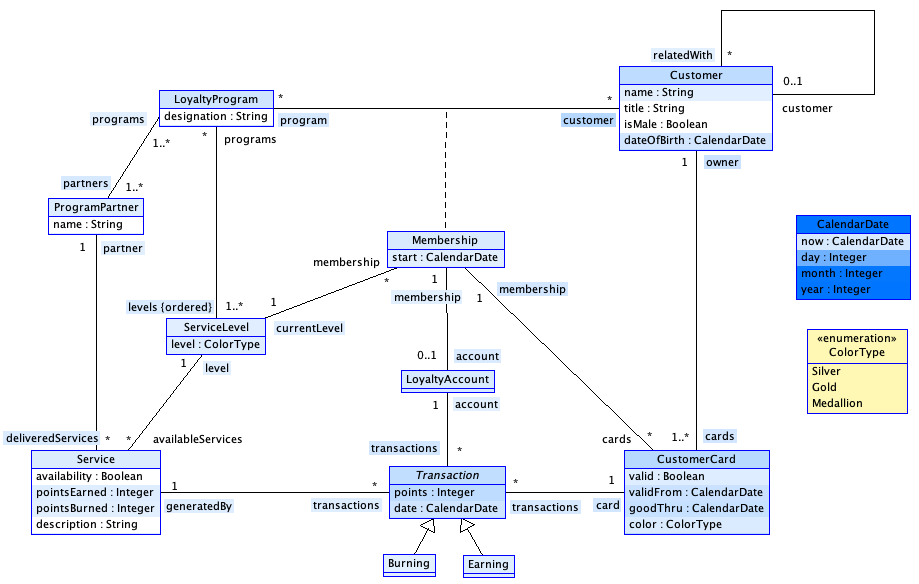
\includegraphics[width=0.9\textwidth]{Chapters/figures/4_RelatedWork/05_USETool_3.png}
\caption{View of class diagram with coverage (Royal and Loyal example from~\cite{Warmer2003})}
\label{fig:05_usetool3}
\end{figure}

As mentioned above, Eclipse OCL is also an important tool to analyze, as it's becoming the most popular OCL tool. It's part of the Eclipse Modeling Project, which focus on supporting model-driven development by presenting a consolidated set of modeling frameworks, tools, and standards implementations. It enables editing, refactoring, code generation, execution, and interactive debugging of OCL constraints, in the context of a class model. The dynamic input and evaluation of OCL expressions can not only be made on the OCL console (see Figure~\ref{fig:07_eclipseocl_1}) but also using the Java~\gls{api}. It also provides a debugger tool (see Figure~\ref{fig:07_eclipseocl_2}) that offers syntax highlighting with error indications, quick fixes, and content assist. Unfortunately, the available documentation doesn't refer syntax highlighting on the UML class diagram, which is the most important topic in the context of this dissertation.

\begin{figure}[ht]
\centering
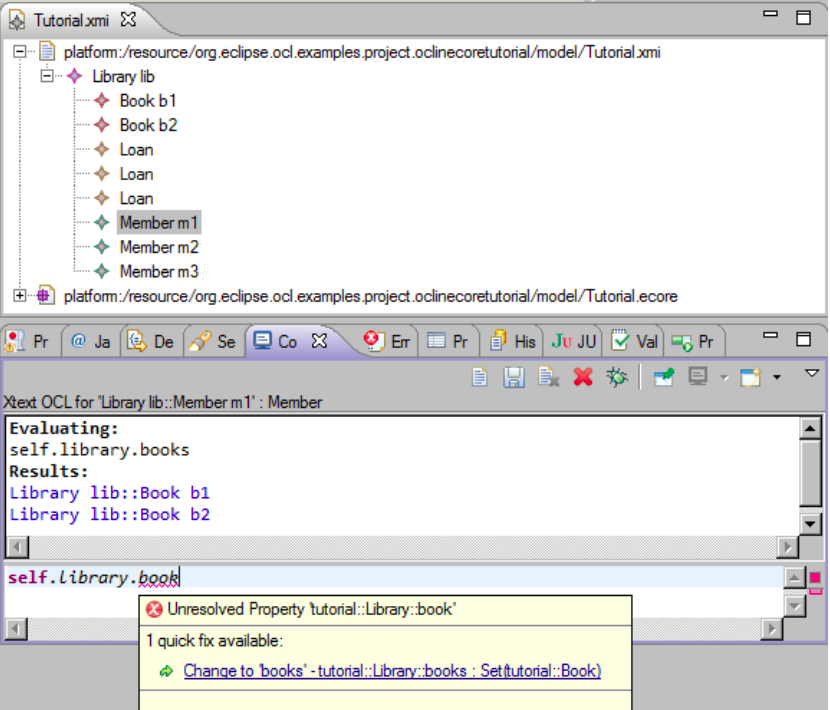
\includegraphics[width=0.7\textwidth]{Chapters/figures/4_RelatedWork/06_eclipseocl_1.png}
\caption{OCL Console~\cite{eclipseocl}}
\label{fig:07_eclipseocl_1}
\end{figure}

\begin{figure}[ht]
\centering
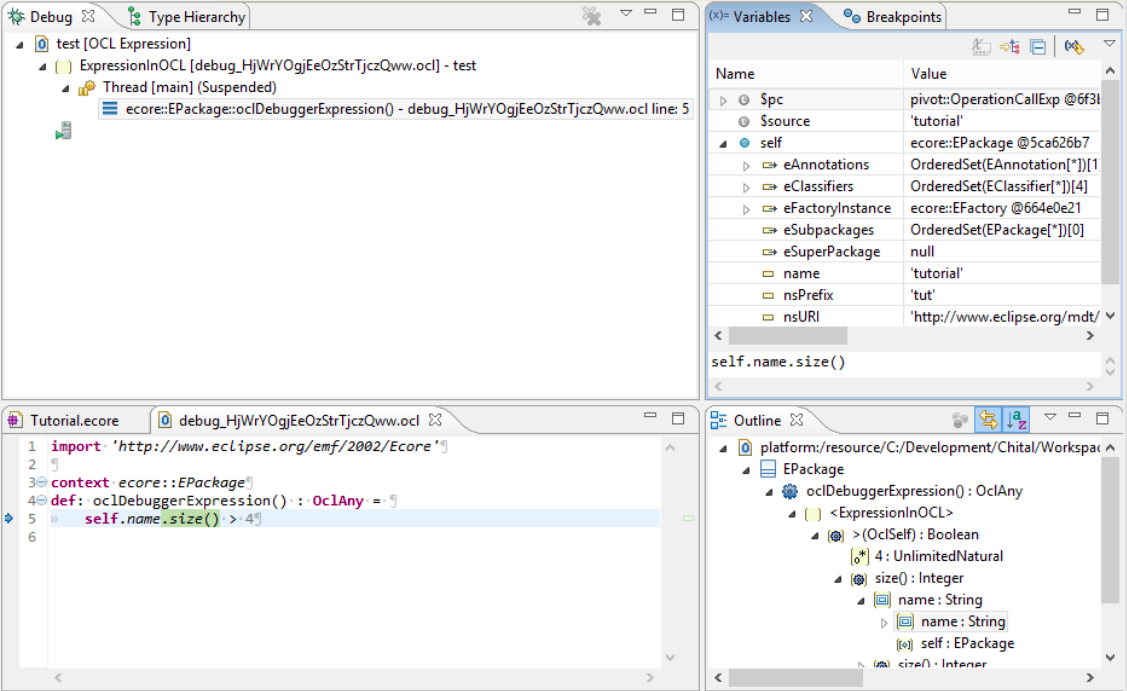
\includegraphics[width=0.7\textwidth]{Chapters/figures/4_RelatedWork/06_eclipseocl_2.png}
\caption{OCL Debugger~\cite{eclipseocl}}
\label{fig:07_eclipseocl_2}
\end{figure}

Both tools offer a wide variety of useful functionalities for modelers, but none provides syntax highlighting on elements of the UML class diagram that are referred on an OCL expression, which we believe that can soften the learning curve of this language. For our research topic, USE is the most relevant tool because it provides the basis for syntax highlighting on the UML class diagram.

%chapter 3
\chaptercover{Prototypes}{chap:Implementation}
{In this chapter, we present the requirements, design and implementation of the two proposed prototypes, from a broader perspective of the component diagram to a detailed description of the implementation details. Section~\ref{chap:Implementation-OCLHighlightPlugin} concerns the OCL Highlight Plugin, followed by Section~\ref{chap:Implementation-OCLComplexityPlugin}, were OCL Complexity Plugin is described.}

As mentioned in previous sections, in this dissertation we propose a tool-based learning feature, dubbed "OCL Highlight Plugin", and an investigation feature, entitled "OCL Complexity Plugin", reified as plugins to Bremen's USE tool. 
Both plugins make use of the same components provided by USE, as presented in the~\gls{componentDiagram} in Figure~\ref{fig:05_componentdiagram}. The concrete implementation of each plugin is described in detail in the following sections.

To make use of these plugins, users should download the corresponding ~\textit{.jar} files (available in each of the corresponding GitHub~\cite{github} repositories indicated below) and place it in the ~\textit{plugins} folder of USE's installation. After restarting USE, two new buttons will show up: clicking on the red marker icon opens the OCL Highlight Plugin, and the green ruler icon will pop-up the OCL Complexity Plugin window. The user should then proceed to import a ~\textit{.usefile} with the definition of the model and a ~\textit{.soil} file with its instantiation (objects). Creating a Class Diagram view is an additional step to make use of the highlight feature.

\begin{figure*}[ht]
    \centering
    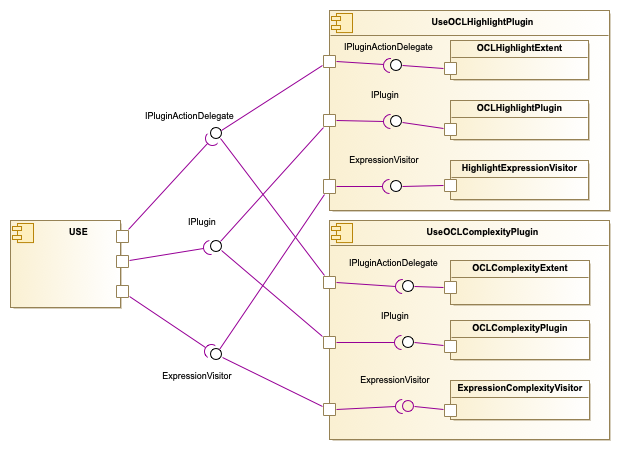
\includegraphics[width=1\textwidth]{Chapters/figures/5_Implementation/ComponentDiagram}
    \caption{OCL Highlight Plugin and OCL Complexity Plugin: Component Diagram}
    \label{fig:05_componentdiagram}
\end{figure*}

\section{OCL Highlight Plugin}
\label{chap:Implementation-OCLHighlightPlugin}

The purpose of the OCL Highlight Plugin is to allow the user to highlight the elements of a UML Class Diagram that are referenced in an OCL expression. These elements include Classes, Attributes, Operations and Relationships. By using strong colours to emphasize the mentioned elements, while painting the rest in lighter colours, we aim to focus the attention of the user on the components that are relevant to the expression under study.

Since USE already includes a coverage option to highlight the elements of the UML Class Diagram that are accessed by each invariant, pre-and post-condition or query operation, the starting point for our work was already in place, speeding up the prototyping phase. The coverage given by USE can be seen in a discriminate way (using the elements browser to select a specific query), or in a integrate way (displaying all the defined queries at the same time). The highlight proposed on this thesis is presented in a dynamic way, whereas in USE  (Gogolla et al.~\cite{GogollaHH14, GogollaHHS15}) it's defined as static (structural coverage when the model is compiled).

\subsection{Requirements}

A set of technical and functional requirements are described for this plugin, not only stating the main functionalities but also some optional yet desired operations that improve its usability. As a technical requirement, it was defined that the plugin should be compatible with USE, meaning that the user can access it's functionalities when working with this tool. In regards to functional requirements, the main use case is that, as a user, I can insert OCL expressions and request the system to highlight it's elements on a Class Diagram. As non-essentials requirements, it was stated that the user could reset the highlighting of the Class Diagram, in order to visualize it as it was initially (default colours defined by USE), and it was suggested that the user could configure the colours of the highlight for each specific element of a Class Diagram (Class, Enum, Attribute, Operation, Rolename and Edge). 
The different use cases defined for this plugin are shown in a Use Case Diagram (Figure~\ref{fig:05_01_usecasediagram}), and typical usage is presented in an Activity Diagram (Figure~\ref{fig:05_01_activitydiagram}).

\begin{figure*}[ht]
    \centering
    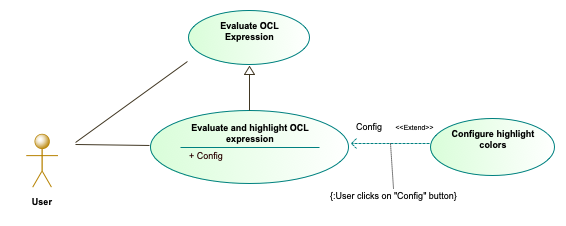
\includegraphics[width=0.9\textwidth]{Chapters/figures/5_Implementation/01_UseCaseDiagram}
    \caption{OCL Highlight Plugin: Use Case Diagram}
    \label{fig:05_01_usecasediagram}
\end{figure*}
    
\begin{figure*}[ht]
    \centering
    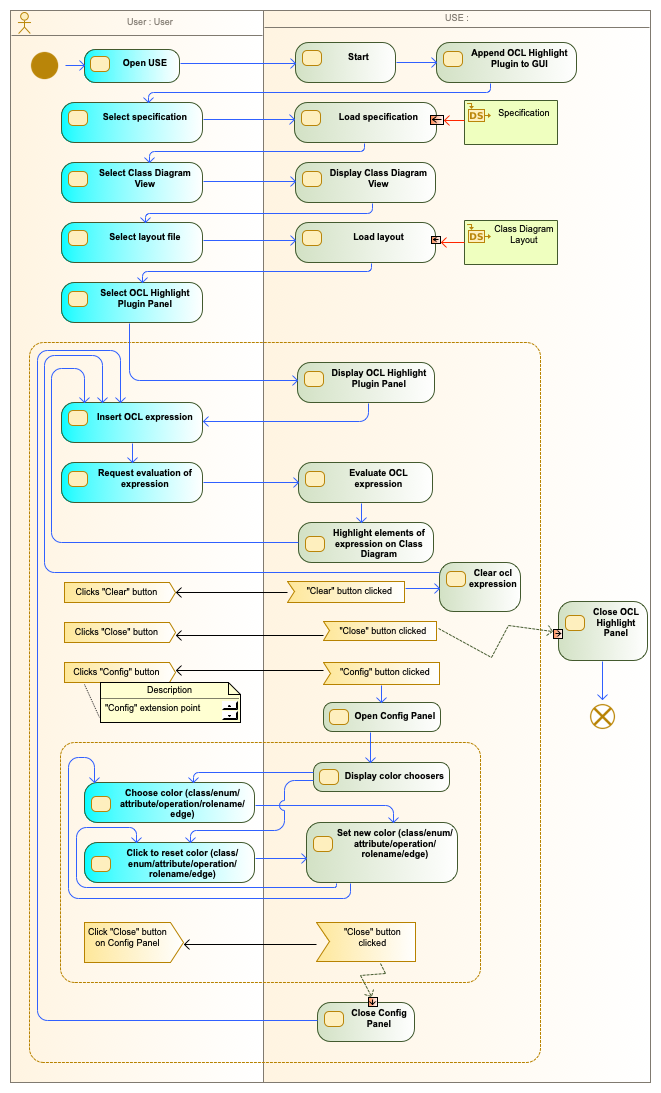
\includegraphics[width=0.9\textwidth]{Chapters/figures/5_Implementation/01_ActivityDiagram}
    \caption{OCL Highlight Plugin: Activity Diagram}
    \label{fig:05_01_activitydiagram}
\end{figure*}

\subsection{Design}

In this subsection, we describe the design of the plugin. Figure~\ref{fig:05_01_classdiagram} presents the Class Diagram, whereas Figure~\ref{fig:05_01_packagediagram} shows the Package Diagram. The implementation of this plugin consisted of the development of the five classes described below: 

\begin{figure*}[ht]
    \centering
    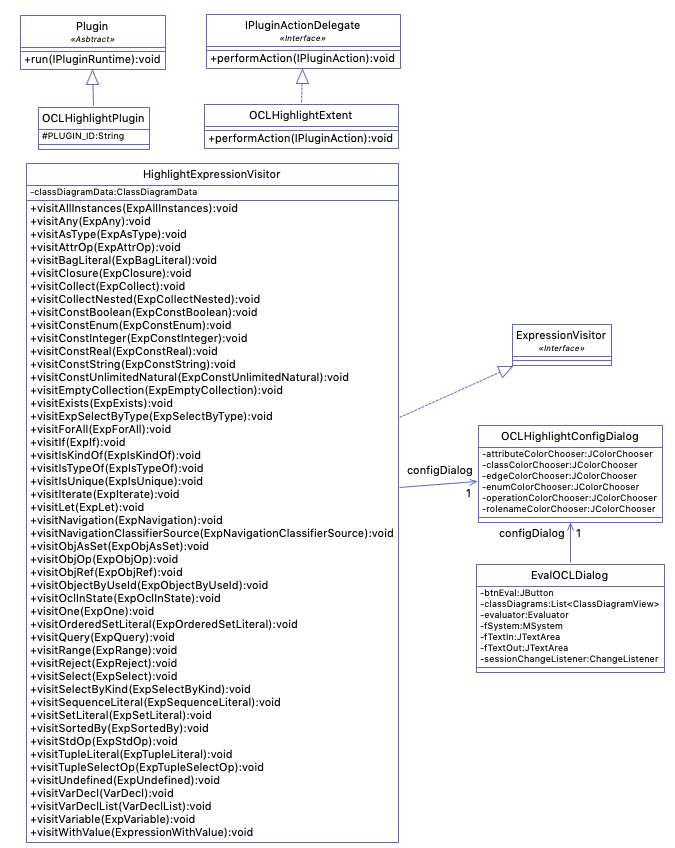
\includegraphics[width=1\textwidth]{Chapters/figures/5_Implementation/01_ClassDiagram}
    \caption{OCL Highlight Plugin: Class Diagram}
    \label{fig:05_01_classdiagram}
\end{figure*}

\begin{figure*}[ht]
    \centering
    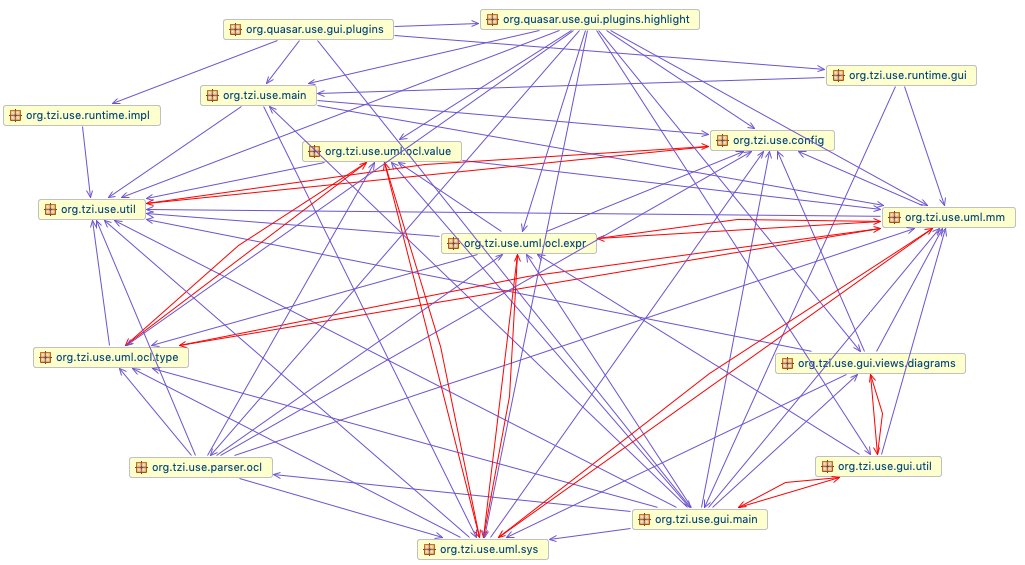
\includegraphics[width=1\textwidth]{Chapters/figures/5_Implementation/01_PackageDiagram}
    \caption{OCL Highlight Plugin: Package Diagram}
    \label{fig:05_01_packagediagram}
\end{figure*}

\textbf{(1) OCLHighlightPlugin:} Main class of the OCL Highlight Plugin. This class defines the id used to identify the plugin. The attribute of this class is shown in Table~\ref{fig:05_01_class1}.

\begin{table}[ht]
\centering
\begin{tabular}{@{}ll@{}}
\toprule
\textbf{Attribute} & \textbf{Description}           \\ \midrule
String PLUGIN\_ID         & Id used to identify the plugin \\ \bottomrule
\end{tabular}
\caption{OCL Highlight Plugin: OCLHighlightPlugin class attributes}
\label{fig:05_01_class1}
\end{table}

\textbf{(2) OCLHighlightExtent:} This is the Plugin Action class. It provides the Action which will be performed if the corresponding Plugin Action Delegate in the application is called. In this case, the Action consists of displaying the panel EvalOCLDialog (with highlight functionality). This class has no attributes.

\textbf{(3) EvalOCLDialog:} This class extends the funcionalities of \textit{JDialog}~\cite{javaxswing}, defining the aspect and actions for entering and evaluating OCL expressions (see Figure~\ref{fig:05_01_panel}), including the creation of text components, labels, and buttons (and their respective action). The attributes of this class are shown in Table~\ref{fig:05_01_class3}. 

\begin{figure*}[ht]
    \centering
    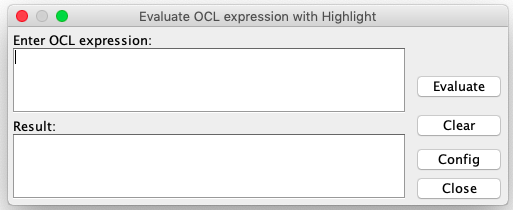
\includegraphics[width=0.8\textwidth]{Chapters/figures/5_Implementation/01_Panel}
    \caption{OCL Highlight Plugin: Panel}
    \label{fig:05_01_panel}
\end{figure*}

\begin{table}[ht]
\centering
\begin{tabular}{@{}ll@{}}
\toprule
\textbf{Attribute}                                         & \textbf{Description}                                                                                                              \\ \midrule
MSystem fSystem                                            & \begin{tabular}[c]{@{}l@{}}Defines the system, including \\ state and functionality\end{tabular}                                  \\ \midrule
JTextArea fTextIn                                          & \begin{tabular}[c]{@{}l@{}}Text area that captures the \\ expression introduced by the user\end{tabular}                          \\ \midrule
JTextArea fTextOut                                         & \begin{tabular}[c]{@{}l@{}}Text area that displays the result \\ of the evaluation of the expression \\ from fTextIn\end{tabular} \\ \midrule
Evaluator evaluator                                        & Evaluates expressions                                                                                                             \\ \midrule
JButton btnEval                                            & Button that triggers the evaluator                                                                                                \\ \midrule
List\textless{}ClassDiagramView\textgreater  classDiagrams & List of the available Class Diagrams                                                                                              \\ \midrule
OCLHighlightConfigDialog configDialog                      & Dialog for configuring highlight colours                                                                                           \\ \midrule
ChangeListener sessionChangeListener                       & \begin{tabular}[c]{@{}l@{}}Change Listener that configures the \\ session of the fSystem\end{tabular}                             \\ \bottomrule
\end{tabular}
\caption{OCL Highlight Plugin: EvalOCLDialog class attributes}
\label{fig:05_01_class3}
\end{table}

\textbf{(4) HighlightExpressionVisitor:} This is the Expression Visitor Class, which implements the methods from the interface \textit{ExpressionVisitor} (available in USE), painting the visited classes of a given OCL expression. The attributes of this class are shown in Table~\ref{fig:05_01_class4}.

\begin{table}[ht]
\centering
\begin{tabular}{@{}ll@{}}
\toprule
\textbf{Attribute}                    & \textbf{Description}                                                                           \\ \midrule
ClassDiagramData classDiagramData     & \begin{tabular}[c]{@{}l@{}}Encapsulates all elements present\\ in a Class Diagram\end{tabular} \\ \midrule
OCLHighlightConfigDialog configDialog & Dialog for configuring highlight colours                                                        \\ \bottomrule
\end{tabular}
\caption{OCL Highlight Plugin: HighlightExpressionVisitor class attributes}
\label{fig:05_01_class4}
\end{table}

\textbf{(5) OCLHighlightConfigDialog:} A dialog for configuring OCL Highlight colours. Similar to EvalOCLDialog, this class extends the funcionalities of \textit{JDialog} (see Figure~\ref{fig:05_01_configcolors}), and defines a set of default colours that can be customized by the user. The attributes of this class are shown in Table~\ref{fig:05_01_class5}.

\begin{figure*}[ht]
    \centering
    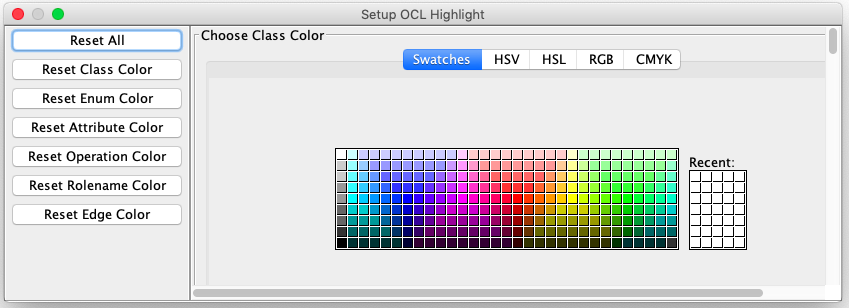
\includegraphics[width=0.8\textwidth]{Chapters/figures/5_Implementation/01_ConfigColors}
    \caption{OCL Highlight Plugin: Highlight colour configuration panel}
    \label{fig:05_01_configcolors}
\end{figure*}

\begin{table}[ht]
\centering
\begin{tabular}{@{}ll@{}}
\toprule
\textbf{Attribute}                                                                                                                                                                           & \textbf{Description}                                                                                                                            \\ \midrule
\begin{tabular}[c]{@{}l@{}}Color CLASS\_COLOR,\\ ENUM\_COLOR,\\ ATTRIBUTE\_COLOR,\\ OPERATION\_COLOR,\\ ROLENAME\_COLOR,\\ EDGE\_COLOR\end{tabular}                                          & \begin{tabular}[c]{@{}l@{}}Default colour for classes, enums,\\ attributes, operations, rolenames, and\\ edge, respectively\end{tabular}  \\ \midrule
\begin{tabular}[c]{@{}l@{}}JColorChooser classColorChooser, \\ enumColorChooser, \\ attributeColorChooser, \\ operationColorChooser,\\ rolenameColorChooser,\\ edgeColorChooser\end{tabular} & \begin{tabular}[c]{@{}l@{}}Colour choosers for classes, enums,\\ attributes, operations, rolenames, and\\ edge, respectively\end{tabular} \\ \bottomrule
\end{tabular}
\caption{OCL Highlight Plugin: OCLHighlightConfigDialog class attributes}
\label{fig:05_01_class5}
\end{table}

\subsection{Implementation}

The OCL Highlight Plugin was developed in Java 8~\cite{java} as an extension for USE. This plugin implements a new OCL evaluation dialog, which resembles the one that is already available in the tool, offering syntax highlighting in the UML Class Diagram when users evaluate a given OCL expression. The OCL expressions are parsed and evaluated using a Visitor pattern~\cite{visitor}, that inherits the functionalities from the interface \textit{ExpressionVisitor} that is made available by USE. After the evaluation, the corresponding UML Diagram elements (such as classes and properties) are highlighted, using a colour that is different to the one provided as default (allowing them to stand out from the rest of the components). Since the API provided by the original tool did not always expose methods and properties to customize the components of the Class Diagram, it was crucial to make the necessary changes using reflection~\cite{reflection}. The concrete implementation of this plugin is available in Github~\cite{useOCLHighlightPlugin}, and a short demo video is accessible in Youtube~\cite{useOCLHighlightPluginDemo}.
 
\subsection{Examples of usage}
\label{chap:Implementation-OCLHighlightPlugin-Examples}

As examples of the behaviour of the plugin, expressions 1 and 2 illustrate the syntax highlighting provided by the evaluation dialog, using the Royal and Loyal model~\cite{Warmer2003}.

\begin{figure*}[ht]
    \centering
    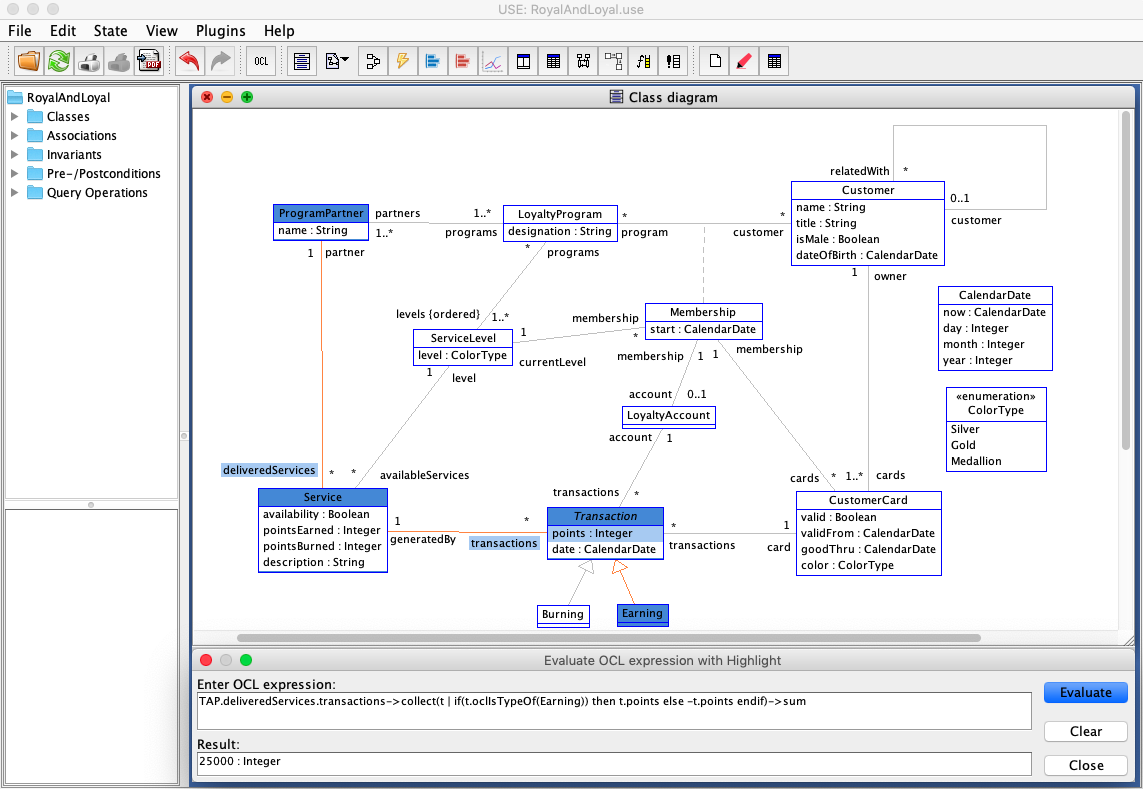
\includegraphics[width=0.94\textwidth]{Chapters/figures/5_Implementation/01_Expression_1}
    \caption{OCL Highlight Plugin: Expression 1}
    \label{fig:01_oclhighlightplugin}
\end{figure*}

\textbf{Expression 1}: This expression exemplifies how to get the balance of points of TAP, which is an instance of \textit{ProgramPartner}. The correspondent highlight is illustrated in Figure~\ref{fig:01_oclhighlightplugin}. The highlighted element are: \textit{ProgramPartner} class, which represents TAP; the navigation from \textit{ProgramPartner} to \textit{Service} (rolename \textit{deliveredServices}), and the \textit{Service} class; and the navigation from \textit{Service} to \textit{Transaction} (rolename \textit{transaction}), and the class \textit{Transaction}. In this expression we want to collect the sum of \textit{points} (property) of a \textit{Transaction}. If a \textit{Transaction} is of type \textit{Earning}, the points are counted positively. If not, they are counted negatively. Both \textit{Earning} and \textit{points} of \textit{Transaction} are also highlighted.

\begin{lstlisting}[caption={OCL expression 1}\label{lst:ocl_expression_1}]
TAP.deliveredServices.transactions
    ->collect(t | if(t.oclIsTypeOf(Earning)) 
        then t.points else - t.points endif)
    ->sum
\end{lstlisting}

\begin{figure*}[ht]
    \centering
    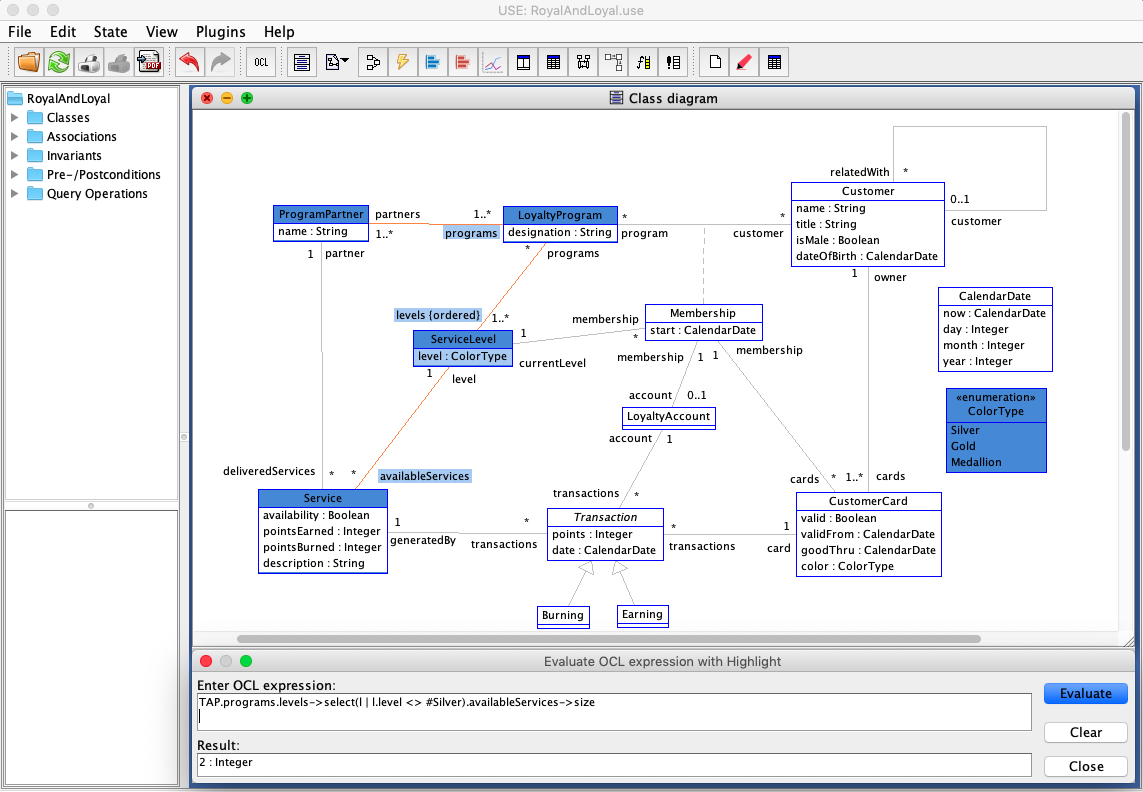
\includegraphics[width=0.94\textwidth]{Chapters/figures/5_Implementation/01_Expression_2}
    \caption{OCL Highlight Plugin: Expression 2}
    \label{fig:02_oclhighlightplugin}
\end{figure*}

\textbf{Expression 2}: This expression exemplifies how to get the number of non-Silver services provided by TAP in the participating Loyalty Programs. The correspondent highlight is illustrated in Figure~\ref{fig:02_oclhighlightplugin}. The highlighted elements are: \textit{ProgramParner}, which again represents TAP; the navigation between \textit{ProgramPartner} and \textit{LoyaltyProgram} (rolename \textit{programs}), and \textit{LoyaltyProgram} class; the navigation between \textit{LoyaltyProgram} and \textit{ServiceLevel} (rolename \textit{levels}), and the class \textit{ServiceLevel}; the \textit{level} (property) of the class \textit{ServiceLevel} and its corresponding type (\textit{ColorType} enum); the navigation from \textit{ServiceLevel} to \textit{Service} (rolename \textit{availableServices}), and the class \textit{Service}.

\begin{lstlisting}[caption={OCL expression 2}\label{lst:ocl_expression_2}]
TAP.programs.levels
    ->select(l | l.level <> #Silver)
    .availableServices->size
\end{lstlisting}

\section{OCL Complexity Plugin}
\label{chap:Implementation-OCLComplexityPlugin}

The second and last plugin presented in this thesis is the OCL Complexity Plugin. As our investigation required to study and analyze several OCL complexity metrics (described in Section~\ref{sec:RelatedWork-Metrics}), we decided to provide them as a plugin, to allow users to evaluate the complexity of the expressions in an automated manner. 

\subsection{Requirements}

This plugin shares the technical requirement with the previous one, meaning that it should be compatible with USE. Regarding functional requirements, we defined that the user should be able to insert OCL expressions and request the computation and display of the complexity of the given expression. To improve the usability, we stated that it should be possible to clear the given expression, allowing the user to easily insert a new one. Additionally, we defined that there should be a panel with a brief explanation of each of the metrics that are displayed, to help the user understand the results of the computation. The different use cases defined for this plugin are shown in a Use Case Diagram (Figure~\ref{fig:05_02_usecasediagram}), and a typical usage is presented in an Activity Diagram (Figure~\ref{fig:05_02_activitydiagram}).

\begin{figure*}[ht]
    \centering
    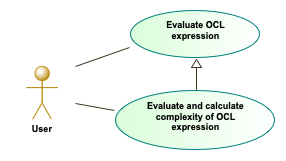
\includegraphics[width=0.6\textwidth]{Chapters/figures/5_Implementation/02_UseCaseDiagram}
    \caption{OCL Complexity Plugin: Use Case Diagram}
    \label{fig:05_02_usecasediagram}
\end{figure*}
  
\begin{figure*}[ht]
    \centering
    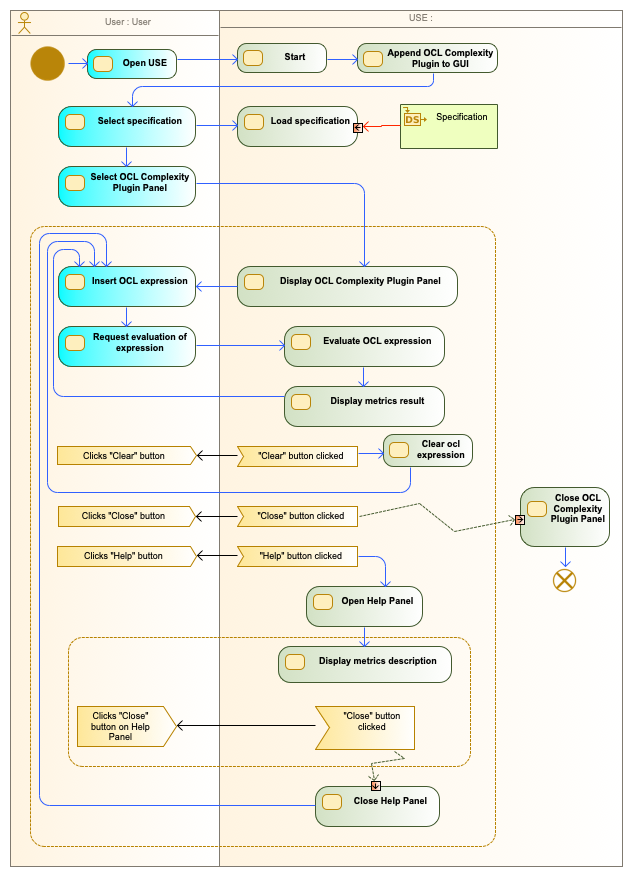
\includegraphics[width=1\textwidth]{Chapters/figures/5_Implementation/02_ActivityDiagram}
    \caption{OCL Complexity Plugin: Activity Diagram}
    \label{fig:05_02_activitydiagram}
\end{figure*}

\subsection{Design}

In this subsection, we describe the design of the plugin. Figure~\ref{fig:05_02_classdiagram} presents the Class Diagram of the implemented system, whereas Figure~\ref{fig:05_02_packagediagram} shows the Package Diagram. The implementation of this plugin consisted of the development of the eight classes and two interfaces described below: 

\begin{figure*}[ht]
    \centering
    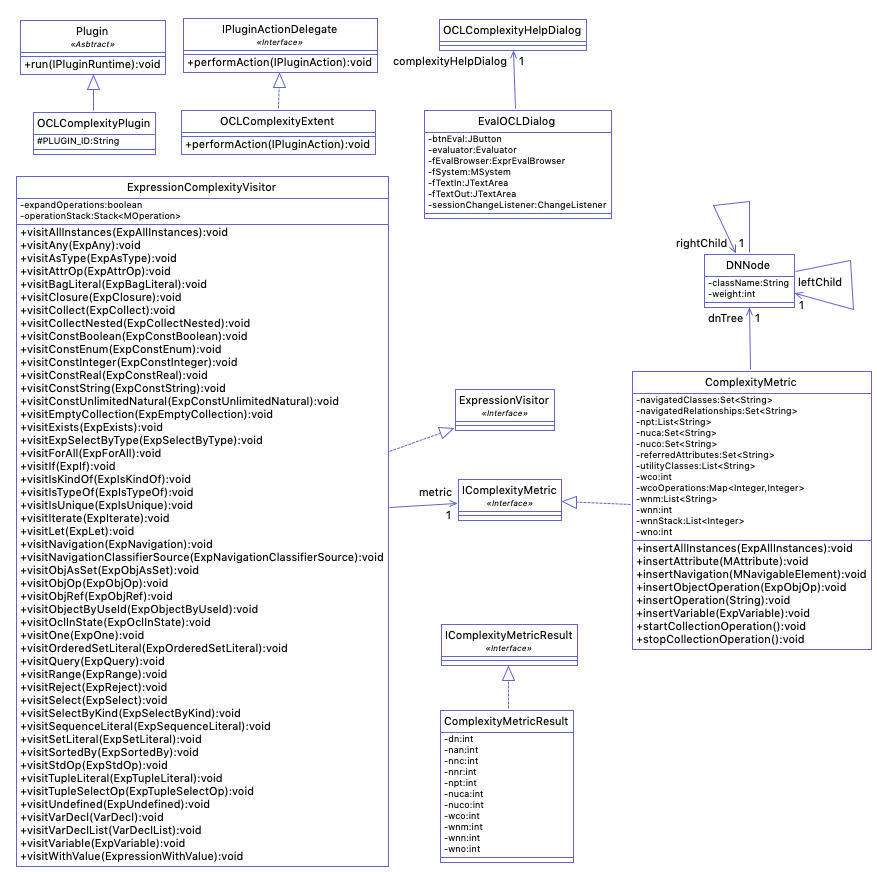
\includegraphics[width=1\textwidth]{Chapters/figures/5_Implementation/02_ClassDiagram}
    \caption{OCL Complexity Plugin: Class Diagram}
    \label{fig:05_02_classdiagram}
\end{figure*}

\begin{figure*}[ht]
    \centering
    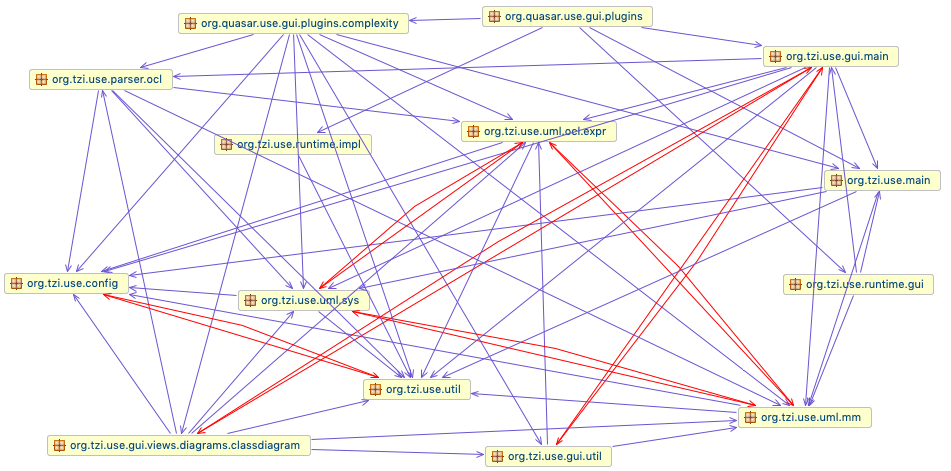
\includegraphics[width=1\textwidth]{Chapters/figures/5_Implementation/02_PackageDiagram}
    \caption{OCL Complexity Plugin: Package Diagram}
    \label{fig:05_02_packagediagram}
\end{figure*}

\textbf{(1) OCLComplexityPlugin:} Main class of the OCL Complexity Plugin. This class defines the id used to identify the plugin. The attribute of this class is shown in Table~\ref{fig:05_02_class1}.

\begin{table}[ht]
\centering
\begin{tabular}{@{}ll@{}}
\toprule
\textbf{Attribute} & \textbf{Description}           \\ \midrule
String PLUGIN\_ID         & Id used to identify the plugin \\ \bottomrule
\end{tabular}
\caption{OCL Complexity Plugin: OCLComplexityPlugin class attributes}
\label{fig:05_02_class1}
\end{table}

\textbf{(2) OCLComplexityExtent:} This is the Plugin Action class. It provides the Action which will be performed if the corresponding Plugin Action Delegate in the application is called. In this case, the Action consists of displaying the panel (with the calculate complexity functionality). This class has no attributes.

\textbf{(3) EvalOCLDialog:} This class extends the funcionalities of \textit{JDialog}~\cite{javaxswing}, defining the aspect and actions for entering and evaluating OCL expressions (see Figure~\ref{fig:05_02_panel}), including the creation of text components, labels, and buttons (and their respective action). The attributes of this class are shown in Table~\ref{fig:05_02_class3}. 

\begin{figure*}[ht]
    \centering
    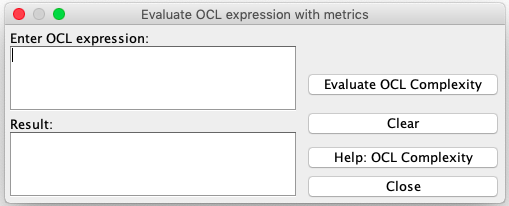
\includegraphics[width=0.8\textwidth]{Chapters/figures/5_Implementation/02_Panel}
    \caption{OCL Complexity Plugin: Panel}
    \label{fig:05_02_panel}
\end{figure*}

\begin{table}[ht]
\centering
\begin{tabular}{@{}ll@{}}
\toprule
\textbf{Attribute}                                        & \textbf{Description}                                                                                                            \\ \midrule
MSystem fSystem                                           & \begin{tabular}[c]{@{}l@{}}Defines the system, including\\ state and functionality\end{tabular}                                 \\ \midrule
JTextArea fTextIn                                         & \begin{tabular}[c]{@{}l@{}}Text area that captures the\\ expression introduced by the user\end{tabular}                         \\ \midrule
JTextArea fTextOut                                        & \begin{tabular}[c]{@{}l@{}}Text area that displays the result\\ of the evaluation of the expression\\ from fTextIn\end{tabular} \\ \midrule
JButton btnEval                                           & \begin{tabular}[c]{@{}l@{}}Button that triggers the complexity \\ evaluation\end{tabular}                                       \\ \midrule
List\textless{}ClassDiagramView\textgreater classDiagrams & List of the available Class Diagrams                                                                                            \\ \midrule
OCLComplexityHelpDialog complexityHelpDialog              & \begin{tabular}[c]{@{}l@{}}Dialog showing an explanation of \\ each complexity metric\end{tabular}                              \\ \midrule
ChangeListener sessionChangeListener                      & \begin{tabular}[c]{@{}l@{}}Change Listener that configures the\\ session of the fSystem\end{tabular}                            \\ \bottomrule
\end{tabular}
\caption{OCL Complexity Plugin: EvalOCLDialog class attributes}
\label{fig:05_02_class3}
\end{table}

\textbf{(4) ExpressionComplexityVisitor:} This is the Expression Visitor Class, which implements the methods from the interface \textit{ExpressionVisitor} (available in USE), calculating the complexity of the expression. The attributes of this class are shown in table~\ref{fig:05_02_class4}. 

\begin{table}[ht]
\centering
\begin{tabular}{@{}ll@{}}
\toprule
\textbf{Attribute}                                    & \textbf{Description}                                                                                         \\ \midrule
Stack\textless{}MOperation\textgreater operationStack & \begin{tabular}[c]{@{}l@{}}Operation stack that controls the navigation\\ on nested operations.\end{tabular} \\ \midrule
IComplexityMetric metric                              & Processes the calculation of metrics.                                                                        \\ \bottomrule
\end{tabular}
\caption{OCL Complexity Plugin: ExpressionComplexityVisitor class attributes}
\label{fig:05_02_class4}
\end{table}

\textbf{(5) ComplexityMetric:} This class calculates and stores the result of the different complexity metrics for an expression. The methods of this class are provided by the interface \textit{IComplexityMetric}, and the attributes are shown in table~\ref{fig:05_02_class5}. 

\begin{table}[ht]
\centering
\begin{tabular}{@{}ll@{}}
\toprule
\textbf{Attribute}                                       & \textbf{Description}                                                                                                              \\ \midrule
Set\textless{}String\textgreater navigatedRelationships  & Set of the navigated relationship names                                                                                           \\ \midrule
Set\textless{}String\textgreater referredAttributes      & Set of the referenced attribute names                                                                                             \\ \midrule
int wno                                                  & Total value of the metric WNO                                                                                                     \\ \midrule
Set\textless{}String\textgreater navigatedClasses        & Set of the navigated classes names                                                                                                \\ \midrule
List\textless{}String\textgreater utilityClasses         & \begin{tabular}[c]{@{}l@{}}List of available utility classes (we \\ only considered "CalendarDate" and \\ "Instant")\end{tabular} \\ \midrule
Set\textless{}String\textgreater nuca                    & \begin{tabular}[c]{@{}l@{}}Set of referenced utility class attribute \\ names\end{tabular}                                        \\ \midrule
Set\textless{}String\textgreater nuco                    & \begin{tabular}[c]{@{}l@{}}Set of referenced utility class operation \\ names\end{tabular}                                        \\ \midrule
int wnn                                                  & Total value of the metric WNN                                                                                                     \\ \midrule
List\textless{}Integer\textgreater wnnStack              & \begin{tabular}[c]{@{}l@{}}Stack of number of operations per depth \\ (on the navigation tree)\end{tabular}                       \\ \midrule
DNNode dnTree                                            & Root of navigation tree                                                                                                           \\ \midrule
Map\textless{}Integer, Integer\textgreater wcoOperations & \begin{tabular}[c]{@{}l@{}}Map of the total of collection operations \\ per depth (on the navigation tree)\end{tabular}           \\ \midrule
int wco                                                  & Total value of the metric WCO                                                                                                     \\ \bottomrule
\end{tabular}
\caption{OCL Complexity Plugin: ComplexityMetric class attributes}
\label{fig:05_02_class5}
\end{table}

\textbf{(6) DNNode:} This class represents a node in the navigation tree. The attributes of this class are shown in table~\ref{fig:05_02_class6}. 

\begin{table}[ht]
\centering
\begin{tabular}{@{}ll@{}}
\toprule
\textbf{Attribute} & \textbf{Description}                      \\ \midrule
String className   & Name of the class represented by the node \\ \midrule
int weight         & Node's weight                             \\ \midrule
DNNode leftChild   & Node's left child                         \\ \midrule
DNNode rightChild  & Node's right child                        \\ \bottomrule
\end{tabular}
\caption{OCL Complexity Plugin: DNNode class attributes}
\label{fig:05_02_class6}
\end{table}

\textbf{(7) ComplexityMetricResult:} This class encapsulates the result of the different complexity metrics for an expression. The methods of this class are provided by the interface \textit{IComplexityMetricResult}, and the attributes are shown in table~\ref{fig:05_02_class7}. 

\begin{table}[ht]
\centering
\begin{tabular}{@{}ll@{}}
\toprule
\textbf{Attribute}                                                                         & \textbf{Description} \\ \midrule
\begin{tabular}[c]{@{}l@{}}int nnr, nan, wno, nnc,\\ nuca, nuco, wnn, dn, wco\end{tabular} & Value of each metric \\ \bottomrule
\end{tabular}
\caption{OCL Complexity Plugin: ComplexityMetricResult class attributes}
\label{fig:05_02_class7}
\end{table}

\textbf{(8) OCLComplexityHelpDialog:} A dialog that displays a short description of each metric. This class extends the functionalities of \textit{JDialog}, with no additional attributes.

\subsection{Implementation}

Similarly to what was described for the OCL Highlight Plugin, this one was also developed in Java 8 as an extension for USE. In this case, the decision to built it for USE instead of another tool was purely based on the fact that, after the development of the first plugin, we already had the knowledge and experience to build an extra functionality for it. The plugins share a similar logic underneath, meaning that they both provide a new evaluation dialog that parses and evaluates expressions using a Visitor pattern. Instead of showing the syntax highlight, this one calculates the complexity metrics of the given expression. The concrete implementation of this plugin is available in Github~\cite{useOCLComplexityPlugin}. In this iteration of the plugin, we decided to exclude the metric WNM, as our models didn't include Messages, and NPT since it's mainly used for pre-and post-conditions, which wasn't part of the questionnaires.

\subsection{Examples of usage}

As examples of the behavior of the plugin, Figure~\ref{fig:02_expression_1} shows the complexity values for Expression~\ref{lst:ocl_expression_1}, whereas Figure~\ref{fig:02_expression_2} presents the values for Expression~\ref{lst:ocl_expression_2} (defined in Subsection~\ref{chap:Implementation-OCLHighlightPlugin-Examples}).

\begin{figure*}[ht]
    \centering
    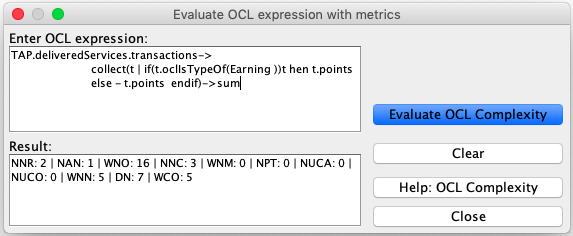
\includegraphics[width=0.8\textwidth]{Chapters/figures/5_Implementation/02_Expression_1}
    \caption{OCL Complexity Plugin: Expression 1}
    \label{fig:02_expression_1}
\end{figure*}

\begin{figure*}[ht]
    \centering
    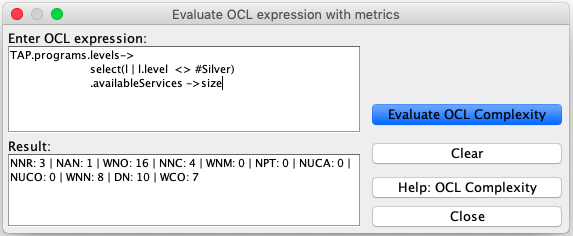
\includegraphics[width=0.8\textwidth]{Chapters/figures/5_Implementation/02_Expression_2}
    \caption{OCL Complexity Plugin: Expression 2}
    \label{fig:02_expression_2}
\end{figure*}


\begin{comment}
1. Requirements
Diagrama de UseCases (descrição em lingua natural com o use case)
- inserir expressao e verificar o highlight
- diagrama de atividades (use cases https://www.modelio.org/)
    duas lanes (utilizador + use)
    
2. Design  
- diagrama de pacotes + diagrama de classes (explicar o que cada classe faz, a sua estrutura, explicar os atributos numa tabela)

3. Implementation
Remeter implementaçao para o github (não é preciso grande descrição)
\end{comment}

%chapter 4
\chaptercover{Experiment and Results}{chap:Results}
{In this chapter, we present several studies conducted during our investigation. In Section~\ref{Results-1} we explore the difficulty of learning OCL when compared to other subjects of SWEBOK, followed by an assessment of the variables that influence students' performance in OCL questionnaires, presented in Section~\ref{Results-2}. Section~\ref{chap:Results-OCLHighlightPlugin} concludes this chapter with the results of the influence of the OCL Highlight Plugin in these same questionnaires.}

\begin{comment}
Experiment 1: Relative Difficulty of Learning OCL
Experiment 2: Assessing OCL Comprehension
    - assessing the success and the duration
    Section 1: Metrics
    Section 2: plugin, model, grades
Experiment 3: On the Effect of Using the OCL Highlight Plugin
 Section 1: avaliação qualitativa dos professores
 Section 2: avaliaçao quantitativa das notas dos alunos
\end{comment}

%explore the concepts and the state of the art concerning the topics that relate to our intended work, which allow us to have a better understanding of the problem under study. This chapter is organized in 5 sections, structured as follows. Section~\ref{RelatedWork-1} starts by presenting the main concepts of Model-Driven Development, including the definition of UML, and OCL. Section~\ref{RelatedWork-2} covers some existing studies on UML class diagrams comprehension, including the impact of OCL on UML-based development. Section~\ref{RelatedWork-3} discusses the complexity of OCL expressions, and how it influences the cognitive effort. Section~\ref{RelatedWork-5} examines, in a broader perspective, relevant papers on the impact of syntax highlighting on program comprehension. Finally, Section~\ref{RelatedWork-5} presents the main OCL support tools and their most important functionalities.


%TODO: some introduction about the context

%We controlled for the origin of students since they were following two different degrees (computer science and business informatics) and the school year since although the overall degree and course syllabus have remained constant during the observation period, variations in students background might have occurred.



%\subsection{Evidence on the Relative Difficulty of Learning OCL}
\section{Experiment 1: Relative Difficulty of Learning OCL}
\label{Results-1}

In this section, we investigate the complexity of learning OCL when compared to a set of other Software Engineering topics offered in two university courses that together span a full school year. The courses' syllabuses were organized according to the following areas of SWEBOK: Software Requirements, Software Design, Software Construction, Software Testing, Software Maintenance, Software Configuration Management, Software Engineering Management, Software Engineering Process, Software Engineering Tools and Methods, Software Quality. Although OCL was taught as part of the Software Design area, it was considered separately in this study. In the Software Design area were kept other topics, namely the one of "Design Patterns".

After taking each area, learning was assessed through comprehensive questionnaires of closed true-false questions, through an e-learning system. Data was collected in two consecutive years, totalling around 150 students enrolled in four computer science-related graduations\footnote{The dataset used in this section is made available at \url{https://doi.org/10.5281/zenodo.4166133}}. Table~\ref{tbl:SWEBOKDescriptiveStatistics} presents descriptive statistics for the grades obtained in OCL and in the topics framed by the SWEBOK knowledge areas. The variability in the number of students per area is due to the fact that the tests for each topic took place throughout the semester, with some dropouts over time. Also, Software Requirements was taken only by students of 1 of the four graduations, and Software Construction was taken only by students of 3 of the four graduations, resulting in a smaller number of cases compared to the other topics.

% Please add the following required packages to your document preamble:
% \usepackage{booktabs}
\begin{table}[h]
\centering
\caption{Descriptive Statistics for the Learning Grades}
 \label{tbl:SWEBOKDescriptiveStatistics}
\resizebox{\textwidth}{!}{
\begin{tabular}{@{}lccccc@{}}
\toprule
\multicolumn{1}{c}{SWEBOK Area}   & N   & Minimum & Maximum  & Mean      & Std. Deviation \\ \midrule
OCL                               & 156 & 0,00\%  & 100,00\% & 50,9179\% & 33,50341\%     \\
Software Engineering Management   & 124 & 0,00\%  & 93,33\%  & 54,2314\% & 22,06163\%     \\
Software Quality                  & 159 & 0,00\%  & 94,44\%  & 54,3902\% & 21,03014\%     \\
Software Requirements             & 59  & 5,00\%  & 100,00\% & 58,1185\% & 21,84444\%     \\
Software Testing                  & 141 & 0,00\%  & 100,00\% & 60,4914\% & 22,06326\%     \\
Software Configuration Management & 133 & 0,00\%  & 100,00\% & 61,8988\% & 19,04061\%     \\
Software Engineering Process      & 132 & 0,00\%  & 95,00\%  & 65,1486\% & 14,14917\%     \\
Software Design                   & 121 & 0,00\%  & 100,00\% & 65,7350\% & 22,70123\%     \\
Software Construction             & 103 & 14,29\% & 100,00\% & 67,7011\% & 21,92754\%     \\ \bottomrule
\end{tabular}
}
\end{table}

\begin{comment}
    \begin{figure}[ht]
    \centering
    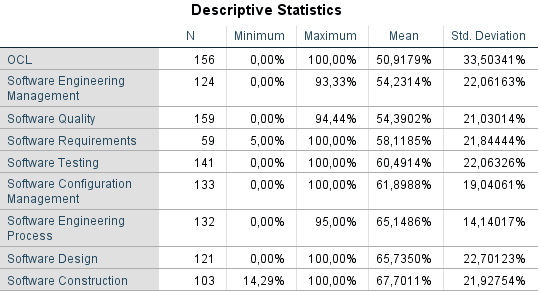
\includegraphics[width=0.8\textwidth]{figures/6_Results/Section1/01_GradesDescriptiveStatistics}
    \caption{Descriptive Statistics for the questionnaire grades}
    \label{fig:GradesDescriptiveStatistics}
    \end{figure}
\end{comment}

OCL was the topic were students obtained the worst grade, on average. To validate if the distribution of grades in OCL is significantly different from the ones obtained in the other topics, we started by performing a One-Sample Kolmogorov-Smirnov Test, with Lilliefors significance correction, to check if the grades obtained in the topics were normally distributed. The results did not allow to assume a normal distribution for most topics. Thus, a non-parametric Related-Samples Wilcoxon Signed Rank Test between the grades obtained in OCL and the remaining areas considered separately was applied. Results are shown in Table~\ref{tbl:OCLvsSWEBOK} for a significance level of 0.05, resulting in the decision of retaining the null hypothesis for Software Requirements, Software Engineering Management, and Software Quality.

\begin{table}[ht]
    \centering
    \begin{threeparttable}  
        \caption{Related-Samples Wilcoxon Signed Rank Test results (questionnaire grades in OCL versus in other SWEBOK topics)}
        
        \label{tbl:OCLvsSWEBOK}
        
        \begin{tabular}{@{}lcl@{}}
            \toprule
            
            SWEBOK Area & Test Sign. & Decision\\
            
            \midrule
            
            Software Requirements & .719 & Retain null hypot.\\
            
            Software Design & .000 & Reject null hypot.\\

            Software Construction & .000 & Reject null hypot.\\

            Software Testing & .011 & Reject null hypot.\\

            Software Maintenance & .026 & Reject null hypot.\\

%            \begin{tabular}[c]{m{3cm}}
                Software Configuration Management
%            \end{tabular}
            & .000 & Reject null hypot.\\

%            \begin{tabular}[c]{m{3cm}}
                Software Engineering Management
%            \end{tabular}
            & .187 & Retain null hypot.\\

            Software Engineering Process & .000 & Reject null hypot.\\

%            \begin{tabular}[c]{m{3cm}}
                Software Engineering Tools and Methods
%            \end{tabular}
            & .006 & Reject null hypot.\\
            
            Software Quality & .487 & Retain null hypot.\\

            \bottomrule
        
        \end{tabular}
        
    \end{threeparttable} 
\end{table}


A Friedman ANOVA test confirmed that there is no significant difference in the distribution of the grades obtained in OCL and in the SWEBOK topics of Software Requirements, Software Engineering Management and Software Quality, $\chi^2\mathrm{p}(3) = 4.86, \rho < 0.05$ (see Figure~\ref{fig:FriedmandANOVA}). 

\begin{figure}[ht]
\centering
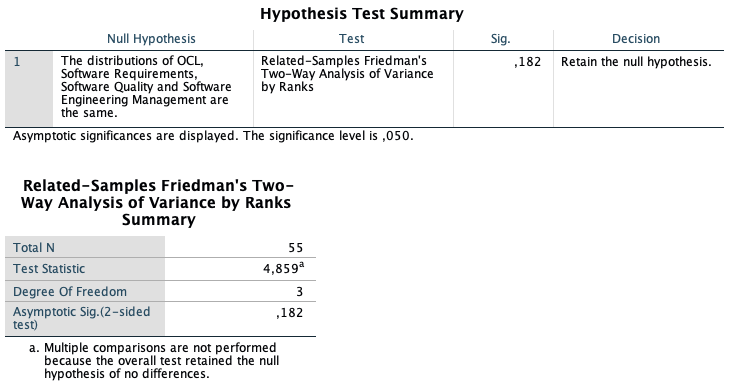
\includegraphics[width=1\textwidth]{Chapters/figures/6_Results/Section1/01_FriedmanANOVA.png}
\caption{Related Samples Friedman ANOVA Test}
\label{fig:FriedmandANOVA}
\end{figure}

From this analysis, we conclude that, despite the claims on OCL being challenging to learn, there are other topics in SWEBOK that reveal similar difficulty. However, as stated in the objectives section, this investigation will is focused on trying to soften the learning curve of OCL.

%\subsection{Analysis of collected data}
\section{Experiment 2: Assessing OCL Comprehension}
\label{Results-2}

\begin{comment}
Experiment 2: Assessing OCL Comprehension
    - assessing the success and the duration
    Section 1: Metrics
    Section 2: plugin, model, grades
\end{comment}   

The analysis presented in this section is based on the dataset\footnote{The collected dataset used in this section is made available at \url{http://xxx}} containing the data collected during five different school years (identified in Figure~\ref{fig:01_barchart_answersperschoolyear} with numbers from 1 to 5). During this five years, students of three different undergraduate university courses were given OCL questionnaires (with a limited duration of 40 minutes) built as follows, to guarantee a true-false answer: the same UML class model with no more than 20 classes (to fit legibly in a computer screen) was made available to all students of a course in advance, and its semantics explained in detail throughout the semester. In the day of the questionnaire, a large set of objects and links were given to students right before they start answering it. Students then instantiate the class model in USE and can make free use of it while answering the questionnaire. Each of its 10 NL questions (extracted randomly from a set of questions, to avoid cheating) could be answered by formulating a quantitative OCL expression upon the instantiated model. For instance, in an instantiated model of Royal and Loyal, the correct answer to \textit{"how many services are provided by TAP?"} would be 42, requiring the students to develop an OCL expression similar to Expression~\ref{lst:ocl_expression_3}. To be considered a correct answer, students had to fill that value in the e-learning platform. In each year, a different UML model was given: FootballCup on years 1 and 3, AirNova on years 2 and 5, and IULTrain on year 4. Models were created with similar complexity (comparable number of classes, including utility classes, and enumerations) to allow a fair assessment across the different school years. It's important to note that on school year 5 the OCL Highlight plugin was introduced to the students, not only for learning during the classes but also as a tool to assist them during the assignments.

\begin{lstlisting}[caption={OCL expression 3}\label{lst:ocl_expression_3}]

TAP.programs.levels.availableServices->size
\end{lstlisting}

\begin{figure}[ht]
\centering
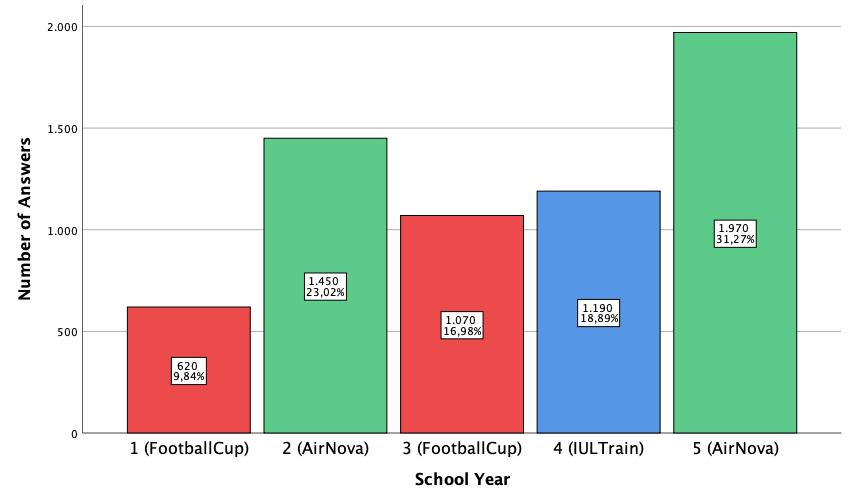
\includegraphics[width=1\textwidth]{Chapters/figures/6_Results/Section2/01_Barchart_AnswersPerYear.jpg}
\caption{Barchart of answers per school year}
\label{fig:01_barchart_answersperschoolyear}
\end{figure}

Figure~\ref{fig:02_barchart_answersperschoolyear} shows a Crosstabs of the percentage of correct answers across the different years. Years 3 and 5 have the highest percentage of correct answers, with 50.1\% and 54.5\% correct answers, respectively. Year 2, despite using the same model as in year 5, showed the smallest value of correct answers, with just 36.3\%. Years 1 and 3 studied the same model (FootballCup), but results don't show a significant difference (only 4\% more correct answers on Year 3, whereas from year 2 to 5 the difference is 18.2\%). 

\begin{figure}[ht]
\centering
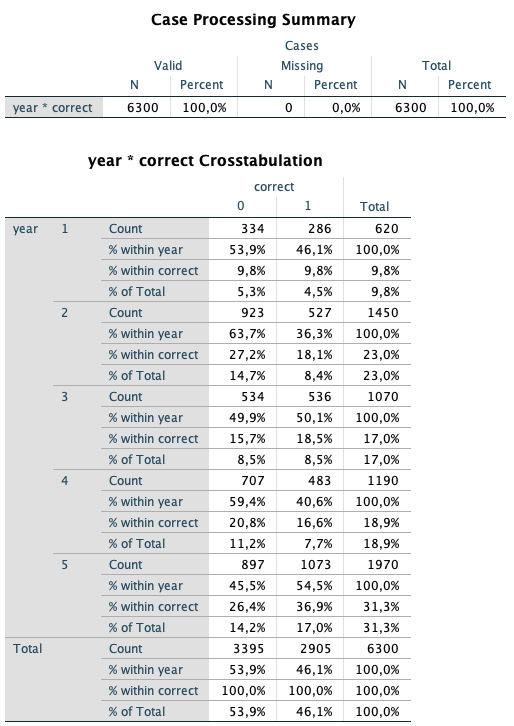
\includegraphics[width=0.7\textwidth]{Chapters/figures/6_Results/Section2/02_CrossTabs_CorrectnessPerYear.png}
\caption{Crosstabs of answers' correctness per school year}
\label{fig:02_barchart_answersperschoolyear}
\end{figure}

In the following subsections we present the studies conducted to analyze the influence of different metrics on the results of student's assessments across the years.

\subsection{OCL complexity metrics}
\label{Results-OCLComplexityMetrics}

As a first attempt, we analyse the influence of OCL complexity metrics on the success rate of student's assessments. From the dataset described above, we extracted the unique OCL expressions, in a total of 140, calculating for each of them its complexities using the OCL Complexity Plugin. Since many metrics were proposed in the literature (Section~\ref{sec:RelatedWork-Metrics}), we executed a variable reduction, not to obtain an overspecified model. 

Using a Kolmogorov-Smirnov test (see Figure~\ref{fig:02_ks_oclmetrics}) we examined the normality of the given metrics. For NNR, the results indicated that OCL metrics do not follow a normal distribution, D(140) = .19, p = .00 (other metrics showed similar results).

\begin{figure}[ht]
\centering
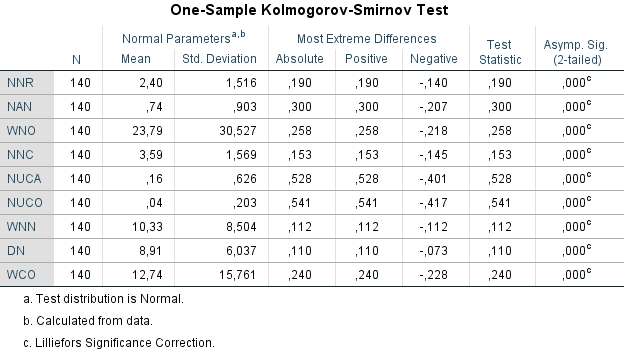
\includegraphics[width=1\textwidth]{Chapters/figures/6_Results/Section2/01_KS_OCLmetrics}
\caption{Kolmogorov–Smirnov test on the normal distribution of OCL complexity metrics}
\label{fig:02_ks_oclmetrics}
\end{figure}

To evaluate if these metrics can explain the success of students answers, and because the independent variables (metrics) don't follow a normal distribution, we applied a Spearman's rho correlation coefficient to evaluate their correlation, and their effect on the dependent variable (student's success). Figure~\ref{fig:01_sr_oclmetrics} presents the result of this test. Our decision was to exclude metrics with strong correlation, as they can be used to explain the same results, keeping the metrics that are more dissimilar (indentified in dark blue). The resulting metrics were NAN, WNO, NUCO, and WCO, as they reveal greater influence on the dependent variable.

\begin{figure}[ht]
\centering
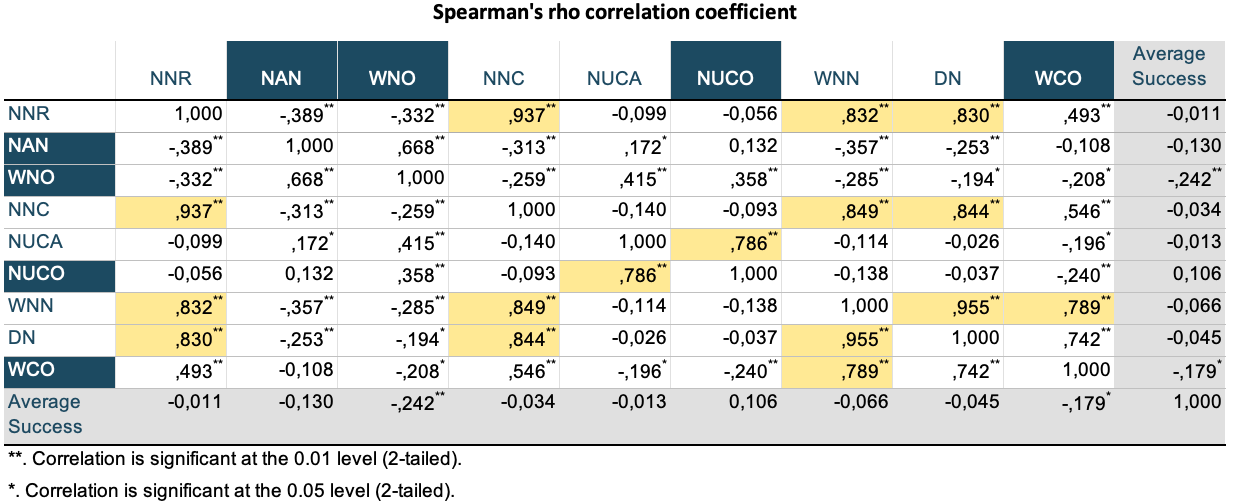
\includegraphics[width=1\textwidth]{Chapters/figures/6_Results/Section2/01_SR_OCLmetrics}
\caption{Spearman's rho correlation coefficient of OCL complexity metrics}
\label{fig:01_sr_oclmetrics}
\end{figure}

After reducing from nine to only four metrics, we performed a Linear Regression to assess the capability of the reduced set to explain the success of the students, as Spearman's rho can evaluate relative monotonies whether the models are linear or not. The results of this test are shown in Figure~\ref{fig:01_lr_oclmetrics}. A significant regression equation was found F(4, 135) = 4.313, $p<.01$, $R^{2}$ = .113, $R^{2}adjusted$ = .087. The resulting linear model revealed a poor explanatory power on the dependent variable (student's success), meaning that there is a monotony relationship, but it is not linear. The regression coefficient $B$ = .041 indicated that an increase in one point in NAN corresponded, on average, to an increase in student's success of .041 points (analogous analysis to other metrics).

\begin{figure}[ht]
\centering
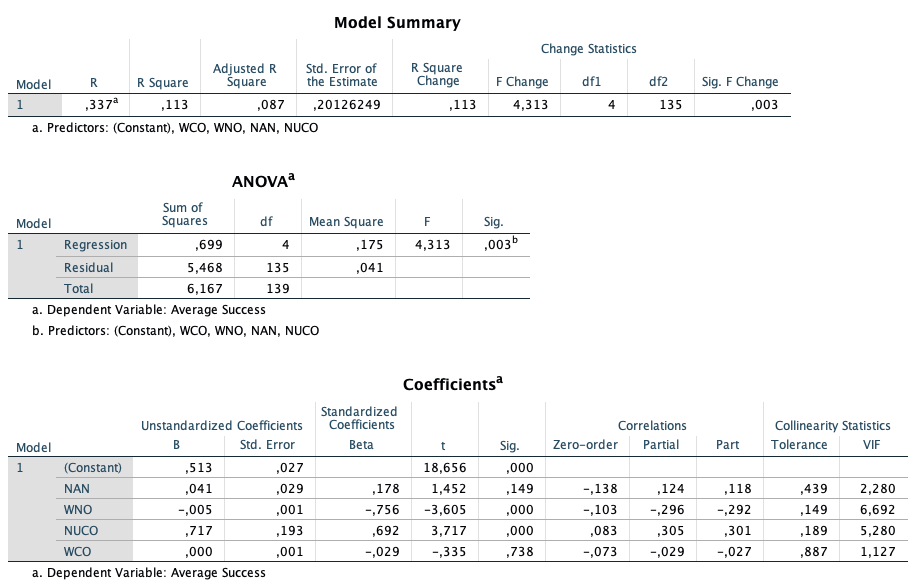
\includegraphics[width=1\textwidth]{Chapters/figures/6_Results/Section2/01_LR_OCLmetrics.png}
\caption{Linear Regression using NAN, WNO, NUCO, and WCO to explain the success}
\label{fig:01_lr_oclmetrics}
\end{figure}

Given the weak results of the first variable reduction, we opted for a Principal Component Analysis on the initial metrics that resulted in three components with a cumulative explanatory power of 90.986\% (Figure~\ref{fig:02_fa_oclmetrics}). The weight of each metric on the components can be seen in Figure~\ref{fig:02_cm_oclmetrics}. 

\begin{figure}[ht]
\centering
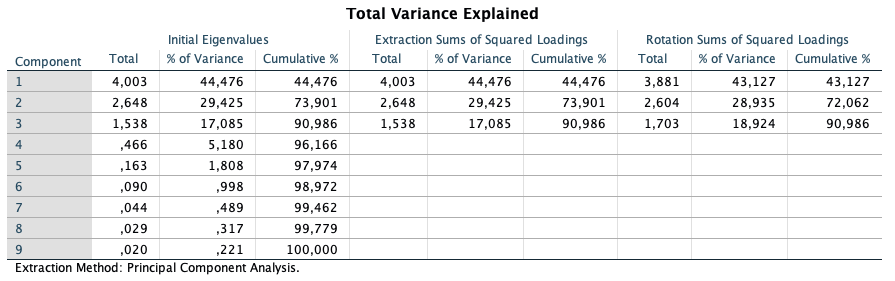
\includegraphics[width=1\textwidth]{Chapters/figures/6_Results/Section2/02_FA_TotalVarianceExplained.png}
\caption{Factor Analysis for OCL metrics}
\label{fig:02_fa_oclmetrics}
\end{figure}

\begin{figure}[ht]
\centering
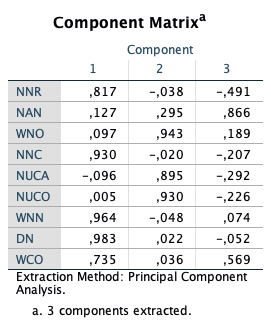
\includegraphics[width=0.35\textwidth]{Chapters/figures/6_Results/Section2/02_FA_ComponentMatrix.png}
\caption{Component Matrix for resulting three components}
\label{fig:02_cm_oclmetrics}
\end{figure}

Using a Binary Logistic Regression, we tried to predict the success of the students considering the three extracted components. Different input methods were tested, but we only achieved very poor results with $R^{2}$ around 3\%.

\begin{comment}

Using a Binary Logistic Regression, we tried to predict the success of the students considering the three extracted components. Different input methods were tested, but we only achieved very poor results with $R^{2}$ around 3\%. Figure~\ref{fig:02_ct_oclmetrics} presents the Classification Table using Forward Stepwise (Likelihood Ratio) method. Prediction for incorrect values showed an acceptable accuracy of 78.8\%, but a weak accuracy of only 24.1\% for the correct values, resulting in a weak prediction percentage of the model of 55.1\%.


\begin{figure}[ht]
\centering
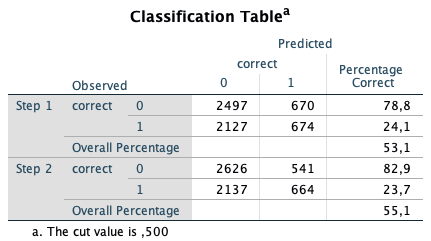
\includegraphics[width=0.5\textwidth]{Template ISCTE-IUL updated/figures/6_Results/Section2/02_FA_ClassificationTable.png}
\caption{Classification table for resulting three components}
\label{fig:02_ct_oclmetrics}
\end{figure}

\end{comment}

The tests described above didn't allow us to conclude that there's a significant correlation between OCL complexity metrics and the success of the students.

\subsection{Readability metrics}

In the previous section, we pursued without success for an explanation of the correctness of students' answers considering the complexity of the solution, i.e., the OCL expression. In this section, we investigate if the explanation can be found instead in the complexity of the problem, i.e., if the complexity of the question posed to the students has a significant influence in the correctness of the responses.

To measure the complexity of the questions, we decided to apply several of the available readability metrics proposed by experts in Literature and Readability over the years~\cite{sanja2013}, which are available in an online tool named Readable~\cite{readable}. For example, for the question \textit{"how many services are provided by TAP?"}, the values for each metric are as seen in Table~\ref{tbl:nlMetricsTap}.

\begin{table}[h]
\centering
\caption{Readability metrics for the given question}
\label{tbl:nlMetricsTap}
\begin{tabular}{@{}ll@{}}
\toprule
Metric                      & Value \\ \midrule
Flesch-Kincaid Grade Level  & 7.4   \\
Gunning Fog Index            & 14.2  \\
Coleman-Liau Index          & 6.0   \\
SMOG Index                 & 11.2  \\
Automated Readability Index & 2.9   \\
FORCAST Grade Level         & 11.4  \\ \bottomrule
\end{tabular}
\quad
\begin{tabular}{@{}ll@{}}
\toprule
Metric                    & Value \\ \midrule
Powers Sumner Kearl Grade & 6.5   \\
Rix Readability           & 6     \\
Flesch Reading Ease       & 54.7  \\
Spache Score              & 3.8   \\
New Dale-Chall Score      & 2.6   \\
Lix Readability           & 36    \\
Lensear Write             & 85.7  \\ \bottomrule
\end{tabular}
\end{table}

Similarly to the OCL complexity metrics, and because we were again facing a high number of variables (total of 13), we decided to assemble a variable reduction. A Kolmogorov-Smirnov test indicates that the majority of the proposed Readability metrics do not follow a normal distribution, D(140) = .089, p = .009 (for Flesch–Kincaid Grade Level, other metrics show similar results). After executing a Spearman’s rho correlation coefficient to evaluate their correlation, and excluding the metrics with strong correlation, we ended up with a smaller set containing the Automated Readability Index, Forest Grade Level, New Dale-Chall, and Lensear Write. Applying a Linear Regression to assess the capability of the resulting metrics to explain the correctness of the answers, a significant regression equation was found F(4, 135) = 6.311, $p<.001$, with an $R^{2}$ of .158. The resulting linear model revealed once again a poor explanatory power on the success of the students.


\begin{comment}
\begin{figure}[ht]
\centering
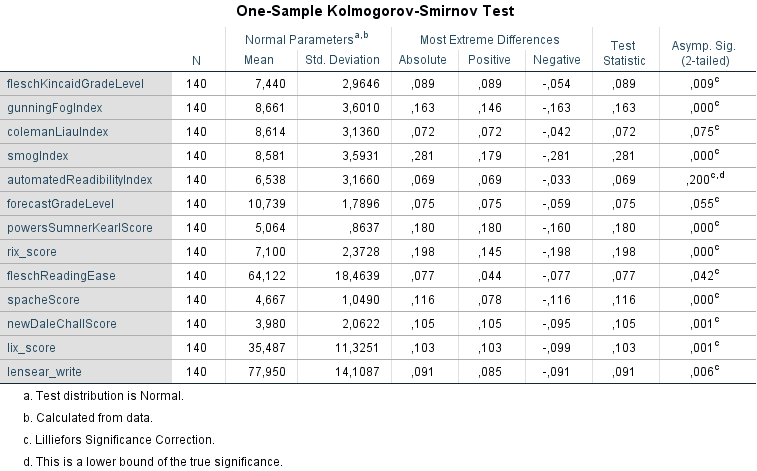
\includegraphics[width=1\textwidth]{Template/Chapters/figures/6_Results/Section2/02_KS_NLmetrics}
\caption{Kolmogorov–Smirnov test on the normal distribution of Readability metrics}
\label{fig:02_ks_nlmetrics}
\end{figure}

\begin{figure}[!h]
\centering
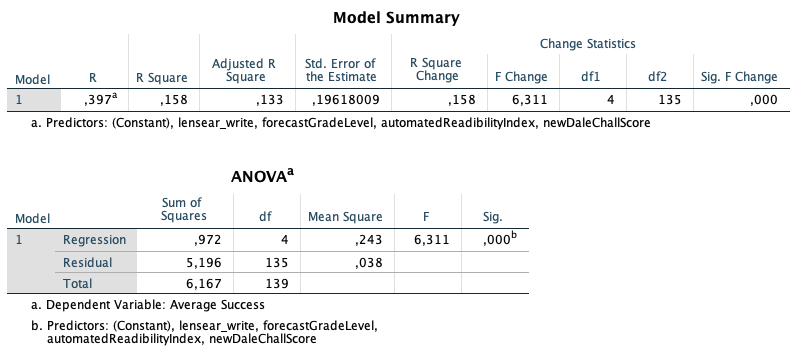
\includegraphics[width=0.48\textwidth]{Figures/SPSS/02_LR_NLmetrics.png}
\caption{Linear Regression using Automated Readability Index, Forest Grade Level, New Dale-Chall, and Lensear Write to explain the success}
\label{fig:02_lr_nlmetrics}
\end{figure}
\end{comment}

In conclusion, our tests show that neither the complexity of the questions, given by Readability metrics, nor the complexity of the answers, given by OCL complexity metrics, can be used to explain the success of the students when answering the questionnaires.

\section{Experiment 3: On the Effect of Using the OCL Highlight Plugin}
\label{chap:Results-OCLHighlightPlugin}

In this last section of experiments, we focus on understanding whether the OCL Highlight Plugin was able to soften the learning curve when studying OCL and therefore produced the desired effect for which it was intended. Before requesting the students to use the plugin on their final questionnaires, it was important to have a stable version. The development of the plugin required several iterations, which allowed for the correction of bugs and also the introduction of “nice-to-have” features, such as the configuration of the highlight colours. The feedback on the stability and usefulness of the plugin was first questioned to experts in the field. After making the necessary corrections, the students were able to experiment with the plugin during the semester. On the day of the exam, we collected their answers, and by comparing the results to the ones obtained in previous school years, we were able to discern the positive impact of the plugin.

\subsection{Qualitative evaluation: experts}
\label{chap:Results-pluginExperts}

In this subsection, we present the focus group study we conducted to obtain feedback and experiences
from UML/OCL experts (teachers) when using the OCL Highlight Plugin to teach OCL to undergraduate students at the university. This experience followed the available guidelines on how to plan and run focus groups~\cite{Kontio2004}:

\paragraph{Defining the research problem:} The objective of the study was to provide insights into the utility of the developed plugin to ease the learning of OCL from the perspective of UML/OCL experts (teachers). Furthermore, we sought to obtain suggestions for improvement and the teachers' opinions on how students reacted to it.

\paragraph{Selecting the participants:} Six teachers from the Department of Computer Science at ISCTE were invited by e-mail to take part in the focus group discussions. The selected invitees are Software Engineering experts, and they teach UML and OCL to bachelor students.

\paragraph{Planning and conducting the focus group session:} We designed the focus group session to consist of two parts. On the first part, teachers were asked to individually observe their respective students during a week of classes, where students were submitted to their first contact with USE and the plugin. At the end of the week, teachers were invited to attend a one-hour meeting to discuss their observations and fill out a previously prepared short questionnaire about the usefulness of the plugin and the reaction of students to it.

\paragraph{Analysis:} Results in Table~\ref{tbl:pluginValidation} indicate that UML/OCL experts agreed on the usefulness of the plugin and that it helps students to understand how OCL transverses a class diagram. This assessment showed that students could easily operate with the plugin, as we did not want to aggravate the difficulty in learning by introducing another element that they would need to manage. As a last remark, some teachers also referred that students thought that the highlighting was something obvious, which again might indicate that it provides a natural integration with the tool.

% Please add the following required packages to your document preamble:
% \usepackage[normalem]{ulem}
% \useunder{\uline}{\ul}{}

%\begin{tabular}{p{0.25\linewidth}p{0.25\linewidth}p{0.25\linewidth}}
\begin{table*}[ht]
\scriptsize
    \centering
    
    \caption{Qualitative Validation of the OCL Highlight Plugin}
    
    \label{tbl:pluginValidation}
    
    \begin{tabular}{cll}
        
        \hline
        
        \\
        
        \multicolumn{1}{l}{}QUESTIONS & 
        %\begin{tabular}[c]{@{}l@{}}
        \begin{tabular}[c]{m{5.5cm}}
            What is your opinion, as a UML/OCL expert, on the usefulness of this plugin? Considering that you have used the tool without the plugin, do you think it can  help students when learning OCL? \\ \\
        \end{tabular}
        
        \begin{tabular}[c]{m{5.5cm}} 
            How did the students in your class(es) react to the plugin? In particular, the assimilation of the visual metaphor was easy, that is the correspondence between the textual expression in OCL and the highlighted elements in the class diagram? \\ \\
        \end{tabular}
        
        \\
        
        \hline
        
        \\
        
        \begin{tabular}[c]{m{1cm}}
            Expert 1
        \end{tabular} &
        
        \begin{tabular}[c]{p{5.5cm}}
            An indispensable and missing plugin, so far! While learning OCL, it is critical to understand the relationship between the often complex OCL expressions and related modeling elements defined in a class diagram – often complex as well. OCL Highlight plugin delivers a simple, yet complete, graphical representation of those relationships, thus facilitating the understanding and learning of OCL expressions.
        \end{tabular}
        
        \begin{tabular}[c]{p{5.5cm}}
            The students quickly understood the usefulness and ease of use of the plugin. The visual matching between the OCL expression and the related modeling elements in the class diagram was considered very intuitive. The graphical feedback also motivated the students to try out and understand increasingly complex OCL expressions.
        \end{tabular} 
        
        \\
        
        \begin{tabular}[c]{m{1cm}}
            Expert 2
        \end{tabular} & 
        
        %\begin{tabular}[c]{@{}l@{}}
        \begin{tabular}[c]{m{5.5cm}}
            I consider that the plugin is of great utility since it illustrates the navigation of the queries in OCL. It facilitates the understanding of the expressions, as well as the understanding of OCL language.
        \end{tabular}
        
        \begin{tabular}[c]{m{5.5cm}}
            The reaction of the students to the plugin was something natural as if it was something obvious that the tool "painted the way". I took the opportunity of asking them if the path was not painted in the class diagram would be more difficult to understand the semantics of queries, and most students said yes.
        \end{tabular}
        
        \\
        
        \begin{tabular}[c]{m{1cm}}
            Expert 3
        \end{tabular} &
        
        \begin{tabular}[c]{m{5.5cm}}
            The plugin is extremely important as students have some difficulties to understand OCL and, more importantly, to build OCL expressions. This visual insight helps to grasp how OCL operates over the model.
        \end{tabular}
        
        \begin{tabular}[c]{m{5.5cm}}
            Yes, they have immediately realized which parts of the model were involved.
        \end{tabular}                                                               
        
        \\
        
                \begin{tabular}[c]{m{1cm}}
            Expert 4
        \end{tabular} &
        
        \begin{tabular}[c]{m{5.5cm}}
            It is a very useful plugin since it helps the students understand what classes are being used in each OCL expression. It introduces traceability and shows a better insight to the students, making it easier for them to learn.
        \end{tabular}
        
        \begin{tabular}[c]{m{5.5cm}}
            Yes, they understood quickly how OCL expressions worked.
        \end{tabular}
        
        \\
    
        \begin{tabular}[c]{m{1cm}}
            Expert 5
        \end{tabular} &
        
        \begin{tabular}[c]{m{5.5cm}}
            This plugin is mostly a good facilitator and a really useful tool for the understanding of UML/OCL, mainly when we have class diagrams with a considerable size. Especially for students, it can ease and improve the process of learning OCL queries.
        \end{tabular}
        
        \begin{tabular}[c]{m{5.5cm}}
            In class and with this plugin, students were able to follow the OCL expressions they were writing by immediately visualizing the result of those queries in terms of the used classes, associations and attributes that were highlighted. Students accepted the use of this tool really well, compared with the previous year, it not only provided a more engaging learning experience for the students but also, as a lecturer, it helped to demonstrate the process of querying.
        \end{tabular} 
        
        \\
        
        \begin{tabular}[c]{m{1cm}}
            Expert 6
        \end{tabular} &
        
        \begin{tabular}[c]{m{5.5cm}}
            I believe that, in fact, this plugin can facilitate the learning of OCL by the students. The selective visualization allows a greater concentration and effectiveness of the analysis of the pathway performed by the queries.
        \end{tabular}
        
        \begin{tabular}[c]{m{5.5cm}}
            The students in my class seemed to assimilate well the connection between the path highlighted in the diagram and the path made by the OCL queries.
        \end{tabular}
        
           \\ \\
        
        \hline
    
    \end{tabular}

\end{table*}


\subsubsection{Quantitative evaluation: students}
\label{chap:Results-pluginStudents}

As a last set of experiments, we explore the impact of the usage of the plugin on students' answers. To consider it a success, we aspire to observe a significant increase in correct answers, when comparing to previous school years where the courses were given without the plugin. We are also interested in observing how the duration of the questionnaires was affected.
For this analysis, we only considered the school years 2 and 5 because they used the same model, in an attempt to isolate the effect of using different models. Since the e-learning platform didn't allow to collect the time the students took per question in year 2 (only the cumulative time of the test was available), we grouped the total of correct answers per test. 
On the matter of test duration, a Levene's test found that the assumption of homogeneity of variance between the groups (test duration and usage of the plugin) was violated, $p<.01$; therefore we carried out a two-tailed independent samples T-Test based on unequal variances. The test duration with plugin (M=2012.91, SD=398.554) is accepted as similar when compared to not using the plugin (M=1942.59, SD=257.579), t(-1.968)=332.825, $p=.05$ (Figure~\ref{fig:03_TTest_Duration}). With a p-value at the limit of rejection, we assume from the calculated average values that the time consumption is very similar, despite being slightly superior when using the plugin.

\begin{figure}[ht]
\centering
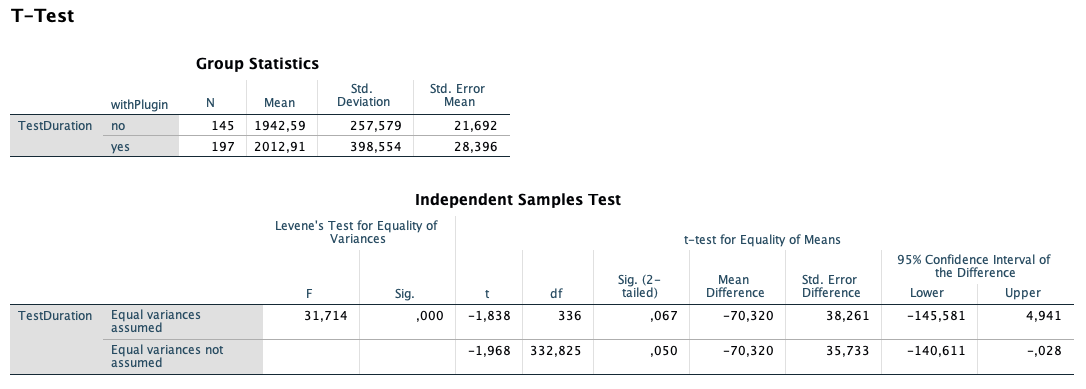
\includegraphics[width=1\textwidth]{Template/Chapters/figures/6_Results/Section3/03_TTest_Duration.png}
\caption{Independent Samples T-Test between test duration and usage of the plugin}
\label{fig:03_TTest_Duration}
\end{figure}

A similar analysis was made, this time considering the correct answers. The equality of variances was met using a Levene’s test, $p>.05$. An independent samples T-Test for equal variances showed that the number of correct answers was significantly higher when using the plugin (M=5.45, SD=2.807) than when not using it (M=3.63, SD=2.879), t(-5.836)=340, $p<.05$ (Figure~\ref{fig:03_TTest_Correct}).


\begin{figure}[ht]
\centering
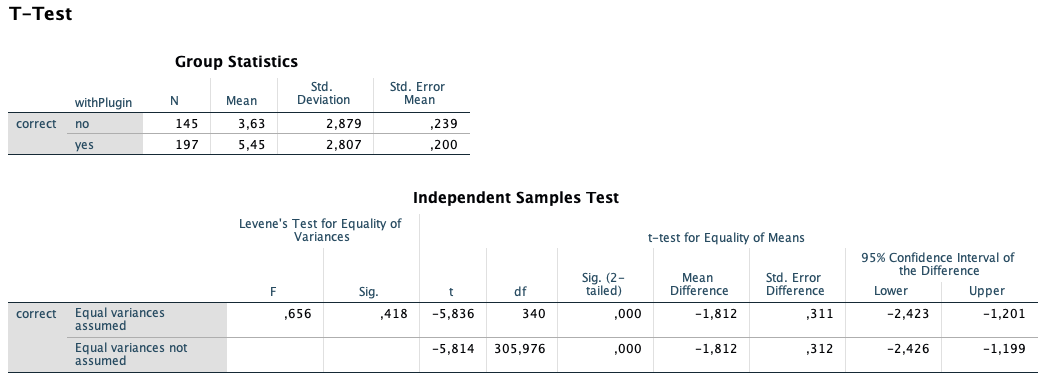
\includegraphics[width=1\textwidth]{Template/Chapters/figures/6_Results/Section3/03_TTest_Correct.png}
\caption{Independent Samples T-Test between total of correct answers and usage of the plugin}
\label{fig:03_TTest_Correct}
\end{figure}

The analyses presented above allow us to conclude that even though there was a slight increase in the amount of time used by the students to complete the questionnaires, it was not significant. On the other hand, the grades (amount of correct answers) revealed a notable improvement. With these tests, we inferred that using the plugin proved to be beneficial to students when learning OCL, and did not introduce an additional effort that would reduce the speed of response of the questionnaires.

A Chi-Square test of independence confirmed this conclusion, showing that there is a significant association between using the plugin and the correctness of the answers, $\chi^{2}$(1, N = 3420) = 110.177, $p<.01$ (Figure~\ref{fig:03_Plugin_Chi_Square_Subset}). We obtained a similar result when performing the same test against the whole dataset (years 1 to 5), $\chi^{2}$(1, N = 6300) = 80.538, $p<.01$.

\begin{figure}[ht]
\centering
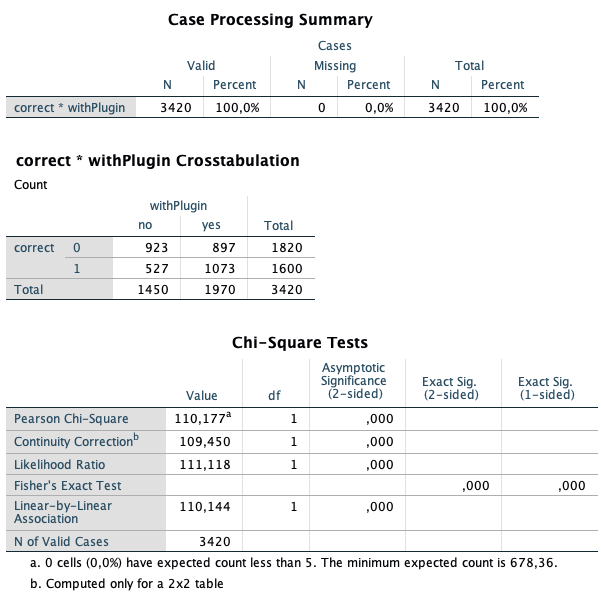
\includegraphics[width=0.7\textwidth]{Template/Chapters/figures/6_Results/Section3/03_Plugin_Chi_Square_Subset.png}
\caption{Chi-Square test for the association between answer's correctness and usage of the plugin}
\label{fig:03_Plugin_Chi_Square_Subset}
\end{figure}

As a last test, it is crucial to prove that there was no difference between the complexity of the questions and answers on both years, as that would jeopardize our experiences. Assuming equal variances between the complexity of the questions in years 2 and 5 (Levene's test with $p>.01$), a T-Test shows that there was no significant difference between the groups, $p>.01$ (see Figure~\ref{fig:03_TTest_NLMetrics}). The same test applied to OCL complexity metrics requires a deeper analysis, as the results for each metric are dissimilar (see Figure~\ref{fig:03_TTest_OCLMetrics}): assuming equal variances for NNR, NNC and DN (Levene's test, $p>.01$), there is no significant difference between both groups, $p>.01$; assuming equal variances for NAN (Levene's test, $p>.01$), complexity of answers in year 2 is significantly higher when compared to year 5, $p<.01, t>0$; assuming unequal variances for WNO, NUCA and WNN (Levene's test, $p<.01$), there is no significant difference between groups, $p>.01$; assuming unequal variances for WCO (Levene's test, $p<.01$), complexity of answers in year 2 is again significantly higher than in year 5, $p<.01, t>0$. 

\begin{figure}[ht]
\centering
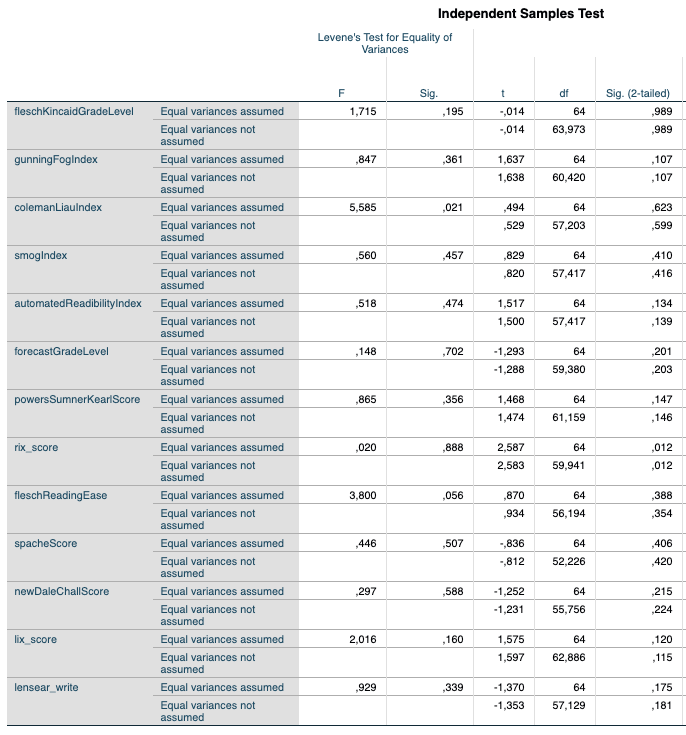
\includegraphics[width=1\textwidth]{Template/Chapters/figures/6_Results/Section3/03_TTest_NLMetrics.png}
\caption{Independent Samples T-Test between the readability metrics of years 2 and 5}
\label{fig:03_TTest_NLMetrics}
\end{figure}

\begin{figure}[ht]
\centering
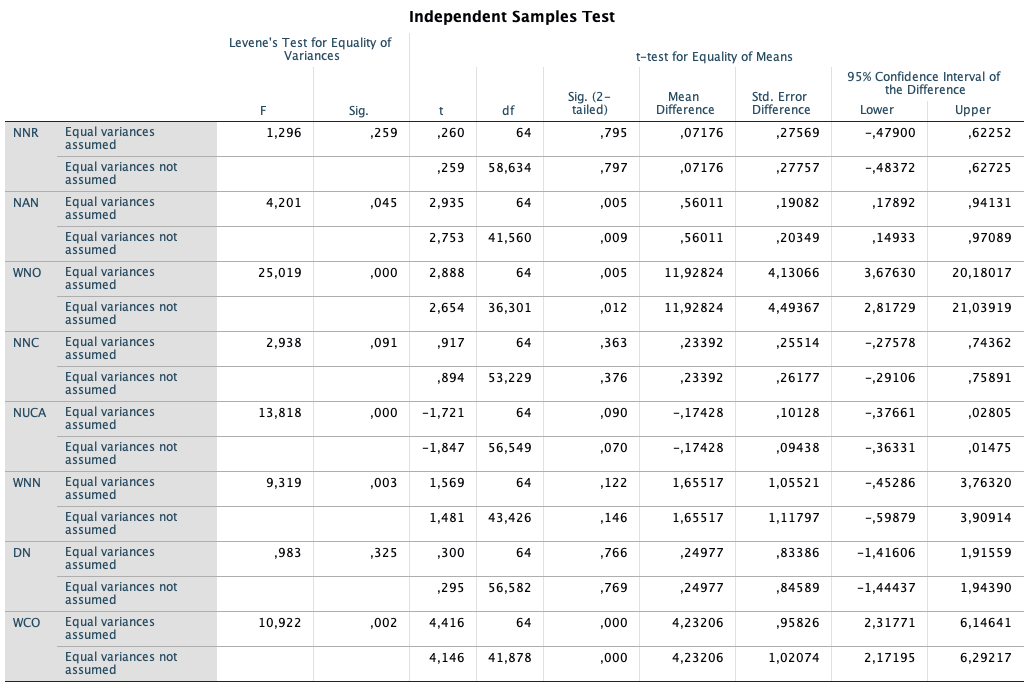
\includegraphics[width=1\textwidth]{Template/Chapters/figures/6_Results/Section3/03_TTest_OCLMetrics.png}
\caption{Independent Samples T-Test between the OCL complexity metrics of years 2 and 5}
\label{fig:03_TTest_OCLMetrics}
\end{figure}

\begin{comment}
An initial chi-square test of independence showed that there is a significant association between using the plugin and the correctness of the answer, $\chi^{2}$(1, N = 6300) = 80.538, $p<.01$ (see Figure~\ref{fig:03_Plugin_Chi_Square}).

\begin{figure}[ht]
\centering
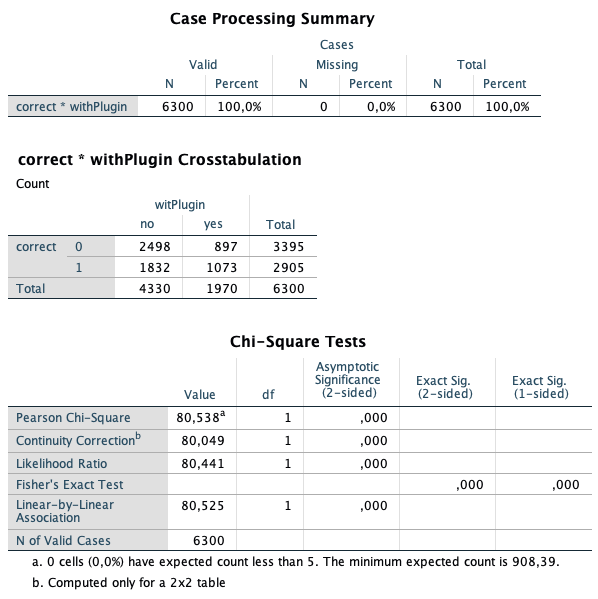
\includegraphics[width=0.7\textwidth]{Chapters/figures/6_Results/Section3/03_Plugin_Chi_Square.png}
\caption{Chi-Square test for the association between answer's correctness and usage of the plugin}
\label{fig:03_Plugin_Chi_Square}
\end{figure}


Our result is statistically significant, i.e, we accept the alternative hypothesis which states that there is a significance association between answer's correctness and usage of the plugin. Correctness is not independent of the usage of the plugin.
$\chi^{2}$(1, N = 6300) = 80.538, $p<.01$
\end{comment}










%chapter 5
\chaptercover{Conclusions and Future Work}{chap:Conclusion}
{In this chapter, we present the verdicts of our experiments, including open issues, limitations, as well as future work directions.}

\section{Discussion}

This dissertation was triggered by claims made in the literature stating that OCL is a topic difficult to learn. We collected data systematically during two consecutive school years, with the help of an e-learning platform, on the outcome of the learning process of a collection of SWEBOK topics, from a large set of undergraduate students, through extensive closed questions questionnaires. OCL appeared in the group of challenging topics, but it did not clearly emerge as the most difficult one.

We also performed inferential statistics to identify the cause of students success/failure in learning OCL, based on similar questionnaires to the ones mentioned above, where students had to translate NL clauses to OCL expressions to answer the questions appropriately. The explanatory variables that we explored were: (i) the linguistic complexity of the questions (problem domain) in NL, ranked by different readability formulas, and (ii) the complexity of the OCL clauses, measured by a set of metrics proposed in the literature, required to answer those questions (solution domain). Neither individually, nor in conjunction, were the aforementioned variables able to provide an acceptable explanatory power, as denoted by low R-squared values in the experiments. 

In addition to shedding light on the factors that influence the OCL learning process, we proposed a tool-based learning feature, dubbed "OCL Highlight", reified as a plugin on the USE tool, which highlights how an OCL clause traverses a UML Class Diagram. We validated this feature by combining an action-research observation period on more than six hundred students in lab sessions, with semi-structured interviews whose conclusions were consolidated by a focus group of experts. We were able to compare the success of students between years where the plugin was used, and the years where it wasn't available. A full consensus was reached that the highlighting feature had a positive effect in the OCL learning process, improving the overall grades without a significant increase in the time needed to complete the OCL questionnaires.

\section{Future Work}

With extensive use of the plugin by students in evaluation moments, we were able to corroborate its utility and confirm that it was beneficial when learning OCL. Nonetheless, we would like to extend this validation with more tests using different models with similar complexity. Future tests should also control for the origin of students since they were following three different graduations (``Computer Science", ``Telecommunications and Computer Engineering" and ``Computer Science and Business Management"). Although the course syllabus has remained constant during the observation period, variations in students background might have occurred.

Additionally, some improvements to the plugin can be considered. First of all, it has many internal USE dependencies (as seen in the Package Diagram). In a future implementation, it would be recommended to use a~\gls{facade} pattern to reduce these dependencies and isolate changes resulting from USE itself. And second, we only considered the utility classes presented in our models. Meaning that, if a new model introduced a different one, it wouldn't be acknowledged, and therefore, not highlighted in the Class Diagram. Therefore, a forthcoming iteration should include an automatic mechanism to detect new utility classes.

\begin{comment}
 We controlled for the origin of students since they were following three different graduations (``Computer Science", ``Telecommunications and Computer Engineering" and ``Computer Science and Business Management") and the school year since, although the course syllabus has remained constant during the observation period, variations in students background might have occurred.

The initial validation of this plugin was beneficial for the detection of bugs, which are planned to be fixed in a future version, along with the inclusion of the most relevant suggestions provided by the experts. Additional experiments are required to corroborate the utility of the plugin, including extensive use by students in evaluation moments. Results of this experiment will indicate if the developed plugin was beneficial, or not, for students to learn OCL. Likewise, we intend to present further evidence on the relative difficulty of learning OCL by collecting and analyzing assessments data from more recent school years. 

%Finally, it is also planned an experimental validation to measure the difference between the physiological effort, using eye-tracking technology (pupils’ fixations and saccades), when developing expressions with and without the plugin. 

- Improvements to the plugin:
(1) How to consider more utilityClasses? We only considered the ones available in our models (how to check them dynamically?)
(2) Implement the metrics WNM and NPT
(3) Tem muitas dependências internas do USE (como se pode ver nos package diagrams). Numa próxima implementação seria recomdavel usar um padrao facade para reduzir as dependencias do plugin ( e para isolar das alteraçoes decorrentes do proprio use)
(4) More tests with different models and expressions

- feature interessante (1): guardar as queries (numa estrutura de anel, para que desse a volta) que foram introduzidas no painel e executadas com sucesso (não interessa guardar lixo intermédio), permitindo que fossem repetidas e feitas variantes
- feature interessante (2): tal como o coverage, ter um botão que mostrasse a coverage de várias queries ao mesmo tempo (para ter uma ideia de quais zonas do modelo já explorei)
\end{comment}

\begin{comment}
Pergunta de discussão:
- o que fazia diferente
- clarificar o trabalho futuro
\end{comment}


\addtocontents{toc}{\vspace{2em}}


%-------BIBLIOGRAFIA---------
%Adicionem as referências em BibTeX ao ficheiro references.bib
\label{References}
\lhead{\emph{References}}  
\bibliographystyle{acm}
%\bibliographystyle{plainurl}
\bibliography{references}
%\printbibliography
\end{document}

%-------ANEXOS---------

\appendix
\appendixpage
\addappheadtotoc

\chapter{Anexo}
\addtocontents{toc}{\vspace{2em}}
\backmatter
%\fancyfoot[LE,RO]{\thepage}
